\documentclass[master=cws,masteroption=ai]{kulemt}
\setup{% Verwijder de "%" op de volgende lijn bij UTF-8 karakterencodering
  inputenc=utf8,
  title={Een gecombineerde calculus voor algebraïsche, scoped en parallelle effecten},
  author={Lander Debreyne},
  promotor={Prof.\,dr.\,ir.\ T. Schrijvers},
  assessor={%TODO
  },
  assistant={Ir. B. van den Berg}}
% Verwijder de "%" op de volgende lijn als je de kaft wil afdrukken
%\setup{coverpageonly}
% Verwijder de "%" op de volgende lijn als je enkel de eerste pagina's wil
% afdrukken en de rest bv. via Word aanmaken.
%\setup{frontpagesonly}

% Kies de fonts voor de gewone tekst, bv. Latin Modern
\setup{font=lm}

% Hier kun je dan nog andere pakketten laden of eigen definities voorzien

% Tenslotte wordt hyperref gebruikt voor pdf bestanden.
% Dit mag verwijderd worden voor de af te drukken versie.
\usepackage[pdfusetitle,colorlinks,plainpages=false]{hyperref}


% Voor wiskundige formules
\usepackage{amsmath}
\usepackage{amsthm}
% pijlen
\usepackage{stmaryrd}
% meer pijlen 
\usepackage{latexsym}
%\includeonly{hfdst-n}
\usepackage{semantic}
\usepackage{soul}
\newcommand{\concat}{\mathbin{{+}\mspace{-8mu}{+}}}
\begin{document}

%TODO
\begin{preface}
  ...
  %Dit is mijn dankwoord om iedereen te danken die mij bezig gehouden heeft.
  %Hierbij dank ik mijn promotor, mijn begeleider en de voltallige jury.
  %Ook mijn familie heeft mij erg gesteund natuurlijk.
\end{preface}

\tableofcontents*

\begin{abstract}
% TODO: schrijf abstract
...
%  In dit \texttt{abstract} wordt een al dan niet uitgebreide
%  samenvatting van het werk gegeven. De bedoeling is wel dat dit tot
%  1~bladzijde beperkt blijft.

\end{abstract}

% Een lijst van figuren en tabellen is optioneel
%\listoffigures
%\listoftables
% Bij een beperkt aantal figuren en tabellen gebruik je liever het volgende:
\listoffiguresandtables
% De lijst van symbolen is eveneens optioneel.
% Deze lijst moet wel manueel aangemaakt worden, bv. als volgt:
% TODO: 
%\chapter{Lijst van afkortingen en symbolen}
%\section*{Afkortingen}
%\begin{flushleft}
%  \renewcommand{\arraystretch}{1.1}
%  \begin{tabularx}{\textwidth}{@{}p{12mm}X@{}}
%    LoG   & Laplacian-of-Gaussian \\
%    MSE   & Mean Square error \\
%    PSNR  & Peak Signal-to-Noise ratio \\
%  \end{tabularx}
%\end{flushleft}
%\section*{Symbolen}
%\begin{flushleft}
%  \renewcommand{\arraystretch}{1.1}
%  \begin{tabularx}{\textwidth}{@{}p{12mm}X@{}}
%    42    & ``The Answer to the Ultimate Question of Life, the Universe,
%            and Everything'' volgens de \cite{h2g2} \\
%    $c$   & Lichtsnelheid \\
%    $E$   & Energie \\
%    $m$   & Massa \\
%    $\pi$ & Het getal pi \\
%  \end{tabularx}
%\end{flushleft}

% Nu begint de eigenlijke tekst
\mainmatter

\chapter{Inleiding} \label{inleiding}
Programmeren omvat het schrijven van instructies die een computer uitvoert om een specifieke taak te volbrengen. Programmeurs schrijven programma's in een programmeertaal, een taal die bestaat uit een set woorden, symbolen en regels. Formele systemen zijn nuttig om de eigenschappen en het gedrag van een programmeertaal te bestuderen. Programmeertaal-calculi bieden een wiskundig kader dat analyse mogelijk maakt om de fundamentele eigenschappen van de taal te begrijpen. Met behulp van abstracte algebra en logische notatie worden de syntaxis, de operationele semantiek en het type-en-effectsysteem van een vereenvoudigde versie van de programmeertaal voorgesteld. De syntaxis beschrijft hoe de woorden en symbolen uit de programmeertaal correct geschreven programma's vormen. De operationele semantiek beschrijft hoe programma's uitgevoerd worden. Het type-en effect-systeem beschrijft hoe de termen in de syntaxis een type krijgen.  

\section{Effecten}
Effecten in programma's zijn interacties met een omgeving buiten de lokale omgeving waarin het programma wordt uitgevoerd. Mogelijke effecten zijn het weergeven van informatie op het scherm, het opslaan van gegevens in een database. In programma's zijn effecten noodzakelijk om het gewenste gedrag te bereiken. Anderzijds kunnen effecten onbedoelde en ongewenste gevolgen hebben. In pure functionele programmeertalen kunnen in principe geen effecten plaatsvinden buiten het uitvoeren van een berekening. Omdat de programmeur geen rekening moet houden met andere effecten kan code geschreven in pure functionele programmeertalen makkelijker te begrijpen en over te redeneren zijn. Deze code verhoogt de productiviteit en verlaagt de kans op fouten. Het puur of vrij van neveneffecten zijn van deze programma's kan limiterend zijn voor de expressiviteit en  het bereiken van het gewenste gedrag. Daarom is het elegant introduceren en correct afhandelen van effecten een belangrijke open vraag in het programmeertaal-onderzoek, in het bijzonder voor functionele programmeertalen. Een goede functionele programmeertaal isoleert, controleert en beheert effecten op een voorspelbare manier. Voor de programmeur maakt een goede functionele programmeertaal het redeneren, uitbreiden, testen en onderhouden van programma's met effecten duidelijk en efficiënt. \emph{Expliciete constructies} voor het redeneren over effecten zijn essentieel om dit doel te bereiken. \newline

\section{Monads en effect handlers}
De meest industrie-relevante aanpak om effecten te modelleren in pure, functionele programmeertalen is de \emph{monad} \cite{Moggi1991}. De bekendste voorbeelden zijn Optional in Java, Result in Rust, en de IO monad en de Maybe monad in Haskell. In Haskell zijn \emph{monad transformers}\cite{Liang1995} populair om modulaire compositie van monads, en bijgevolg effecten, te realiseren. Dit gebeurt door verschillende types monads te combineren tot een enkele, gecombineerde monad. \newline 
Een tweede constructie om effecten te modelleren is het gebruik van \emph{algebraïsche effecten \cite{Pretnar2015} en effect handlers}. Het concept is om de aanroep van het effect, of de syntaxis, te scheiden van de afhandeling van het effect, of de semantiek. Een effect handler kan worden beschouwd als een functie die verantwoordelijk is voor de afhandeling van een effect in een andere functie zodat dit op een voorspelbare en modulaire manier kan gebeuren. 

\section{Programmeertaal-onderzoek en industrie}
WebAssembly \cite{Haas2017} is een goed voorbeeld van hoe principes en vooruitgang uit programmeertaal-onderzoek vertaald kunnen worden naar een industrie-relevante programmeertaal. WebAssembly is van het begin af aan ontworpen met een formele semantiek hetgeen bewijst dat dit een waardevolle aanpak kan zijn. De doelen die de auteurs vooropstellen voor een veilige, snelle, draagbare en compacte taal zijn toepasbaar op het ontwerp van bijna alle talen. Met deze principes in gedachte kan toegewerkt worden naar een calculus voor effect handlers die, mits verder ontwikkeling, kan evolueren naar een industrie-relevante aanpak om in een pure functionele taal met effecten om te gaan. Dit met als doel de programmeur een volwaardig alternatief te bieden voor monads in pure, functionele talen. \newline

Een online bibliografie\footnote{\url{https://github.com/yallop/effects-bibliography}} verzamelt toepassingen en applicaties die gerelateerd zijn aan onderzoek rond  op deze manier programmeren met computationele effecten. Koka \cite{Leijen2017}, Eff \cite{Bauer2015} en Effekt \cite{Brachthauser2020} zijn onderzoeks-programmeertalen ontwikkeld met als doel programmeren met effect handlers. De Haskell-library \emph{fused-effects} \footnote{\url{https://github.com/fused-effects/fused-effects}} biedt functionaliteit om in haskell programma's te maken met effect handlers. Deze library wordt gebruikt door Github in de semantic\footnote{\url{https://github.com/github/semantic}} library. Verder is er de Pyro \cite{bingham2019pyro} library voor flexibel en schaalbaar diep probabilistisch programmeren die volgens de auteurs gebouwd is op Poutine, een library om te programmeren met effect handlers, voor de flexibiliteit en separation of concerns die de aanpak met zich meebrengt.

\section{Gecombineerde calculus}
De meest bestudeerde vorm van effect handlers zijn de handlers die algebraïsche effecten behandelen\cite{Bauer2015}. Algebraïsche effecten zijn effecten die geschreven kunnen worden in de vorm $\textbf{op}\ v\ (y.\ c)$ met $v$ een parameter voor het effect en $(y. \  c)$ voor de continuatie of de rest van het programma na het effect. Een reden waarom deze vorm het meest bestudeerd is, is omdat deze effecten generisch kunnen sequencen en forwarden. \newline
Generische sequencing: 
\begin{equation}
    \inference{}{\textbf{do} \  x \leftarrow \textbf{op} \  l \  v \  (y. \  c_1); \   c_2 \leadsto \textbf{op} \  l \  v \  (y. \   \textbf{do} \  x \leftarrow \  c_1 ; \  c_2)}[E-DoOp]
\end{equation} 
Generische forwarding met h een handler die de operatie met label l niet behandelt:
\begin{equation}
    \inference{(\textbf{op}\:l\:\_\:\_) \notin h}{h \star \textbf{op}\:l\:v\:(y.\:c_{1}) \leadsto \textbf{op}\:l\:v\:(y.\: h \star c_{1})}[E-FwdOp]
\end{equation} 
Calculi van effect handlers zouden ideaal gezien drie eigenschappen moeten bezitten.
\begin{itemize}
    \item Overloading van de effecten: De effecten krijgen een verschillende semantiek door het schrijven en gebruiken van verschillende handlers voor hetzelfde programma.
    \item  Functie compositie: Het modulair combineren van verschillende effecten en effect handlers is mogelijk zonder strikte beperkingen.
    \item Effectinteracties: Effecten interageren met elkaar, waarbij de volgorde van de verschillende handlers een rol speelt en nieuwe semantische mogelijkheden biedt.
\end{itemize}

Het scheiden van operaties en hun behandeling, respectievelijk in de effecten en de handlers, zorgt voor overloading en modulaire compositie. Effectinteracties resulteren uit de compositie van niet-orthogonale effecten. \newline

Algebraïsche effect handlers zijn expressief beperkt in de zin dat ze geen model zijn voor alle computationele effecten. Dit vloeit rechtstreeks voort uit de syntaxis van algebraïsche effecten die als input enkel een parameter en de continuatie van het programma hebben waardoor het semantische domein beperkt is. De expressiviteit van programmeren met algebraïsche effect handlers is beperkt als gevolg hiervan. \newline

Het toevoegen van scoped effecten verhoogt de expressiviteit van een effect handler-gebaseerde programmeertaal. Scoped effecten splitsen het programma in een computatie in scope en een deel dat buiten de scope valt. Het resultaat is dat de handler deze continuatie in scope anders kan behandelen dan de computatie out of scope. Deze syntaxis laat complexere semantiek toe door het mogelijk te maken de computatie in scope een andere betekenis te geven dan de  continuatie. Generisch is de syntaxis te schrijven als $\textbf{sc}\:v\:(y.\:c_1)\:(z.\:c_2)$ met $v$ de parameter, $(y.\:c_1)$ de berekening in scope en $(z.\:c_2)$ de continuatie. De $\lambda_{sc}$ calculus \cite{Bosman2022} beschrijft een calculus voor algebraïsche en scoped effecten. Deze is expressiever dan een calculus voor enkel algebraïsche effecten. De $\lambda_{sc}$ calculus behandelt effecten echter strikt sequentieel en laat daardoor mogelijke performantieverbeteringen naast zich liggen. \newline

Methodiek toevoegen om effecten in parallel te behandelen kan de efficiëntie verbeteren. Parallelle algebraïsche effecten\cite{Xie2021} bieden deze mogelijkheid. De $\lambda^{p}$ calculus maakt parallelle afhandeling van effecten mogelijk door gebruik te maken van een parallelle \emph{for each constructie die effecten parallel behandelt} en levert zo mogelijk performantieverbeteringen voor parallelliseerbare algebraïsche effecten. \newline

\section{Doel}
Het doel van deze masterproef is het afleveren van een calculus met effect handlers die een formeel systeem modelleert met ondersteuning voor algebraïsche en scoped effecten en parallelle afhandeling van effecten. In de literatuur bestaat een leemte voor systemen die deze combinatie expliciet ondersteunen. Deze masterproef wil een ontwerp aanreiken voor een dergelijke calculus. Het resulterende ontwerp steunt op een sterke theoretische basis door een formele syntax, semantiek en type-en effectsysteem af te leveren maar kent ook praktische bruikbaarheid door de implementatie van een functionele interpreter. \newline

De beoogde calculus heeft minimaal volgende meta-eigenschappen: 
\begin{itemize}
    \item \emph{Veilig} voor het programmeren met effecten door het schrijven van overzichtelijke en duidelijke programma's mogelijk te maken door scheiding van syntax en semantiek van effecten door gebruik van de effect handler aanpak.
    \item \emph{Snel} door parallelle afhandeling van effecten mogelijk te maken.
    \item \emph{Compact} door een minimale calculus voor te stellen die aan deze eigenschappen voldoet.
    \item \emph{Draagbaar} door een calculus voor te stellen die wijd implementeerbaar is.
\end{itemize}

 De onderzoeksvraag voor deze masterproef luidt: \newline

\emph{Hoe kan een compacte calculus worden gedefinieerd die sequentiële en parallelle afhandeling van algebraïsche en scoped effecten modelleert met behoud van handler overloading, modulaire compositie en effect interacties?}

\section{Overzicht}
Hoofdstuk \ref{hoofdstuk:achtergrond} geeft meer achtergrondinformatie over de onderwerpen die deze masterproef behandelt. Vervolgens overloopt \Cref{hoofdstuk:startpunt} de literatuur waarop deze thesis voortbouwt. De motivatie voor dit onderwerp en de uitdagingen zijn het onderwerp van \Cref{hoofdstuk:motivatie}. De hoofdstukken die daarop volgen vormen de bijdrage van deze masterproef en stellen de $\lambda_{sc}^{p}$-calculus voor met de syntaxis in \Cref{hoofdstuk:syntaxis}, de operationele semantiek in \Cref{hoofdstuk:semantiek}, het type-en effect-systeem in \Cref{hoofdstuk:typesysteem}, voorbeelden in \Cref{hoofdstuk:voorbeelden} en de metatheorie in \Cref{hoofdstuk:metatheorie}. Vervolgens geeft hoofdstuk \Cref{hoofdstuk:evaluatie} een evaluatie van de masterproef, \Cref{hoofdstuk:gerelateerd} geeft een overzicht van gerelateerd werk. Tot slot bevat \Cref{besluit} de conclusie.

%%% Local Variables: 
%%% mode: latex
%%% TeX-master: "masterproef"
%%% End: 
\newtheorem{theorem}{Theorem}[section]
\newtheorem{lemma}[theorem]{Lemma}

% syntaxis van Eff hier?

\chapter{Achtergrond}
\label{hoofdstuk:achtergrond}
Het doel van dit hoofdstuk is om de lezer een introductie te bieden aan enkele onderwerpen die essentieel zijn als achtergrondinformatie om de rest van de masterproef te begrijpen.

\section{Effecten en handlers} \label{sec:achtergrondAlgEff}
Effecten en handlers \cite{Bauer2015} zijn een mechanisme om effecten gestructureerd te behandelen in een programmeertaal. Ze stellen de programmeur in staat om de pure, functionele code in een programma te scheiden van de impure, effectvolle code. Dit gebeurt door effect-operaties te introduceren die effectvolle primitieven zijn. Vervolgens definieert de aanpak specifieke functies, effect handlers, voor het afhandelen van de effect-operaties. Effecten en handlers maken het makkelijker over de logica van de code te redeneren en effecten te coderen en te manipuleren op een modulair componeerbare manier, waardoor meer modulaire en herbruikbare programma's kunnen worden gemaakt. Dit is bijzonder interessant in systemen met complexe effecten of systemen waar werken met effecten niet triviaal is zoals gedistribueerde systemen. \newline

Handlers beschrijven de instructies die de machine uitvoert wanneer een effect optreedt in de controlestroom van het programma. Doordat de semantiek van het effect in de handler zit, is er een scheiding tussen het voorkomen van het effect en de afhandeling, wat redeneren over en controleren van de effecten in een programma vergemakkelijkt. \newline

De belangrijkste eigenschap van programmeren met effect handlers is de hoge mate van modulariteit en diversiteit van semantiek die de programmeur kan bereiken met dezelfde bouwstenen. Dit vloeit voort uit overloading van effecten via verschillende handlers, modulaire compositie van effecten en scheiding van syntax en semantiek bij de afhandeling van effecten. Deze eigenschappen maken dit een veelbelovende aanpak voor het programmeren met effecten. 

\section{Algebraïsche operaties}
De algebraïsche effect-operaties of effecten of operaties hebben een type-signatuur $A \rightarrowtriangle B$. Dit duidt aan dat het effect een term van type A omvormt naar type B. Het $choose:() \rightarrowtriangle Bool$ effect is een voorbeeld van een algebraïsch effect dat een eenheids-waarde neemt als input en een boolean waarde teruggeeft. In de voorbeelden in deze thesis is de boolean waarde die het effect teruggeeft willekeurige of niet-deterministisch. Het gemodelleerde effect van \emph{choose} is met andere woorden non-determinisme. De syntaxis voor het choose effect in deze masterproef is als volgt:

\begin{equation}
    \textbf{op} \: choose \: (\:) \: (y. \: c)
\end{equation}

Hier geeft het sleutelwoord \textbf{op} aan dat het om een algebraïsch effect gaat, gevolgd door het label \textit{choose}, gevolgd door de input parameter $(\:)$, gevolgd door de resumptie $(y. \: c)$. De resumptie is de computatie die de rest van het programma bevat gegeven de resulterende waarde van het effect. Een voorbeeld programma, gebaseerd op een gelijkaardig voorbeeld in \cite{Bosman2022}, met het \textit{choose} effect is een programma dat ''pasta'' of ''pizza'' teruggeeft afhankelijk van het resultaat:

\begin{equation}
    c_{ND}\:=\:\textbf{op}\:choose\:()\:(x.\:then\:return\:"pasta"\:else\:return\:"pizza"\:)
\end{equation}

Algebraïsche effecten worden gekenmerkt door de eigenschap dat ze aan elkaar gerijgd kunnen worden door gebruik te maken van de algebraïciteits-eigenschap als volgt:

\begin{equation} \label{eq:algFood}
    \begin{split}
        \textbf{do}\:food \leftarrow \textbf{op}\:choose\:()\:(x. \: if \: x \:then\:return\:"pasta"\:else\:return\:"pizza"\:) \: ; \\ \: \textbf{return}\: "We \: are \: eating \: " \concat  food \concat " \: tonight!"  \leadsto \\
        \textbf{op}\:choose\:()\:(x.\: \textbf{do}\:food \leftarrow  if \: x \:then\:return\:"pasta"\:else\:return\:"pizza"\:; \\ \: \textbf{return} "We \: are \: eating \: " \concat  food \concat " \: tonight!" )
    \end{split}
\end{equation}

Generisch opgesteld, ziet deze eigenschap er zo uit:

\begin{equation}
    \textbf{do}\:x \leftarrow \textbf{op}\:l\:v\:(y.\:c_{1})\:;\:c_{2} \leadsto  \textbf{op}\:l\:v\:(y.\: \textbf{do}\:x \leftarrow c_{1}\:;\:c_{2})
\end{equation}

Het effect van deze eigenschap is enerzijds dat de \textbf{do} clausule wordt doorgeschoven naar de continuatie en anderzijds dat de computatie na de het \textbf{do} statement (de $c_2$ computatie) in de continuatie wordt geduwd.

\section{Algebraïsche effect handlers}
Het voorbeeld-programma $c_{ND}$ uit is niet te evalueren aangezien de operatie nog geen semantiek heeft in dit programma.
De effect handlers geven semantiek aan de algebraïsche operaties door te definiëren hoe de operaties te interpreteren. Effect handlers hebben drie interessante eigenschappen, overloading van effecten, functie compositie en effectinteracties.

\subsection{Overloading van effecten}
Overloading van effecten is simpel te demonstreren door twee verschillende handlers te definiëren en deze hetzelfde programma te laten behandelen. Het resultaat zal in beide gevallen anders zijn, wat aangeeft dat handlers een interessante invloed hebben op de semantiek van het programma. Het onderstaande voorbeeld is gebaseerd op een gelijkaardig voorbeeld in \cite{Bosman2022}. \newline 
De handler $h_{True}$ selecteert de $true$ tak van de computatie voor het \textit{choose} effect:
\begin{equation}
    \begin{split}
        h_{True} = \textbf{handler} \: & \{ \: \textbf{return}\:x \mapsto \textbf{return}\:x \\
         & , \: \textbf{op}\:choose\:\_\:k \mapsto k \: true\}
    \end{split}
\end{equation}
Deze handler toegepast op het programma uit Eq. \ref{eq:algFood} heeft als resultaat
\begin{equation}
    "We\:are\:eating\:pasta\:tonight!"
\end{equation} 
De handler $h_{Max}$ selecteert beide takken en combineert het resultaat:
\begin{equation}
    \begin{split}
        h_{True} = \textbf{handler} \: & \{ \: \textbf{return}\:x \mapsto \textbf{return}\:[x] \\
        & , \: \textbf{op}\:choose\:\_\:k \mapsto \textbf{do}\:t \leftarrow k \: true\;;\: \textbf{do}\:f \leftarrow k\:false\;\:t \concat f \}
    \end{split}
\end{equation}
Deze handler toegepast op het programma uit Eq. \ref{eq:algFood} zal als resultaat
\begin{equation}
    ["We\:are\:eating\:pasta\:tonight!",\:"We\:are\:eating\:pizza\:tonight!"]
\end{equation} 
hebben. Deze twee resultaten zijn een interessante toepassing van overloading van effecten door verschillende handlers te definiëren voor hetzelfde effect.

\subsection{Functie compositie}
\label{subsec:funcComp}
Functie compositie betekent dat het mogelijk moet zijn om programma's te schrijven die verschillende effecten bevatten. De paper "Effect Handlers in Scope"\cite{Wu2014} stelt dat het bij samenstelling van operaties essentieel is dat niet alleen compositie van de syntaxis van effecten maar ook van hun semantiek triviaal is. Een goed voorbeeld hiervan is hoe in een programma met de orthogonale effecten van state en niet-determinisme de semantiek van het programma kan veranderen door de volgorde van de handlers om te wisselen. Voorbeelden voor deze eigenschap zijn moeilijk om duidelijk aan te tonen op een beknopte manier. Het voorbeeld dat hieronder is beschreven is deels overgenomen van \cite{Wu2014} maar niet het hele voorbeeld is weergegeven. Het voorbeeld bestaat uit het knapsack probleem. Dit probleem bestaat uit het vullen (met vervanging) van een rugzak tot een bepaald gewicht, de eerste parameter, gebruikmakend van een lijst van gewichten, de tweede parameter. De output is een lijst van de gebruikte gewichten. In het voorbeeld is \emph{solutions} de handler die alle mogelijke geldige oplossingen teruggeeft als een lijst. \emph{runState} is een handler die een state van het programma kan opvragen en een nieuwe state kan opslaan. Deze twee handlers resulteren in twee mogelijke evaluatie volgorden: 

\begin{equation}
    runLocal = solutions \  . \   runState \   s
\end{equation}

\begin{equation}
    runGlobal = runState \  . \   solutions \   s
\end{equation}

runLocal geeft een lijst van waarden uiteindelijke waarden terug met voor elke een state. runGlobal geeft een lijst van oplossingen met een globale state. Met \emph{choices} een handler die voor elke keuze de state incrementeert krijgen we volgende programma's:

\begin{equation}
    \begin{split}
        (run \  . \   runGlobal \  (0 :: Int) \   choices) \  (knapsack \   3 \  [3,2,1]) \\
        \leadsto (12,[[3],[2,1],[1,2],[1,1,1]])
    \end{split}
\end{equation}

\begin{equation}
    \begin{split}
        (run \  . \   runLocal \  (0 :: Int) \   choices) \  (knapsack \   3 \ 
  [3,2,1]) \\
        \leadsto [(1,[3]),(5,[2,1]),(5,[1,2]),(9,[1,1,1])]
    \end{split}
\end{equation}


\subsection{Effect-interacties}
\label{subsec:effInter}
Interessante semantiek kan ook bekomen worden door niet-orthogonale effecten te combineren. Dit resulteert in effect-interacties. Deze eigenschap is eveneens moeilijk beknopt te illustrereten. Een voorbeeld van de eigenschap is uitgeschreven in de sectie "Cut and Call" in "Effect Handlers in Scope"\cite{Wu2014} en dit voorbeeld wordt hier beschreven. Om de interactie te beschrijven is het voldoende om het bestaan van een \emph{once} effect te veronderstellen dat de computatie afbreekt bij het vinden van de eerste oplossing. Dit effect heeft duidelijk een interactie met het non-determinisme effect uit de choices handler in het voorbeeld in \ref{subsec:funcComp}. De combinatie van deze twee resulteert in een interactie tussen twee niet-orthogonale effecten. 

\section{Beperkingen algebraïsche effecten en handlers}
Algebraïsche effecten en handlers zijn beperkt in hun vermogen om bepaalde soorten effecten te modelleren. Ze kunnen effecten modelleren zoals onder andere I/O, het veranderen van de staat van variabelen en niet-determinisme. Algebraïsche effecten kunnen echter geen effecten voorstellen die de controlestroom van een programma veranderen, zoals uitzonderingen (geen catch functionaliteit mogelijk). Deze beperking is rechtstreeks terug te brengen naar de syntaxis van de effecten die enkel een parameter en een continuatie hebben. In het geval van een catch functionaliteit is een computatie in scope nodig die als de \emph{try block} van een uitzondering kan gezien worden welke onmogelijk is af te leiden uit enkel de continuatie. Zonder deze try block is het onmogelijk voor de handler om de state van het programma terug te zetten naar de state voor de uitzondering (indien gewenst) om resumptie te doen na de afhandeling (indien gewenst). Buiten catch functionaliteit vereisen andere controlestroom-veranderende effecten ook meer verfijnde mechanismen voor hun behandeling, die buiten de mogelijkheden van algebraïsche effecten vallen. Een categorie van zulke effecten die binnen de scope van deze thesis valt zijn de scoped effecten in Sectie \ref{hoofdstuk:AchteffScope} en de parallelle effecten in Sectie \ref{hoofdstuk:AchteffPar}. Enkele andere categorieën effecten worden besproken in Sectie \ref{subsec:OthCompEff}

\section{Effecten met scope} \label{hoofdstuk:AchteffScope}
Scoped effecten \cite{Bosman2022}, \cite{Wu2014}, \cite{Yang2022}, \cite{Pirog2018} zijn effecten waarbij het gedrag in scope beperkt is tot een deel van de totale berekening. Dit type effect verdeelt het programma in een computatie die binnen het bereik van het effect valt en een deel dat buiten het bereik valt. De $\lambda_{sc}$ calculus \cite{Bosman2022} beschrijft een calculus voor algebraïsche en scoped effecten. De syntaxis en semantiek van deze calculus wordt beschreven in Sectie \ref{hoofdstuk:startpuntScoped}. De syntaxis van scoped operaties ziet er als volgt uit:
\begin{equation}
    \textbf{sc}\:l\:v\:(y.\:c_{1})\:(z.\:c_{2})
\end{equation}

Hier geeft het sleutelwoord \textbf{sc} aan dat het om een scoped effect gaat, gevolgd door een label $l$, een input parameter $v$, een berekening in scope $(y.\:c_{1})$ en een resumptie $(z.\:c_{2})$. Het verschil met de algebraïsche effecten is de toevoeging van een berekening in scope. Deze toevoeging laat de handler toe om de bereking in scope anders te interpreteren dan de resumptie. Door deze toevoeging kan ook geen generieke forwarding van effecten door verschillende handlers meer gebeuren en moet de handler een expliciete forwarding clausule hebben van de volgende vorm:
\begin{equation}
    \textbf{fwd}\:f\:p\:k \mapsto c_{f}
\end{equation}
Sectie \ref{hoofdstuk:startpuntScoped} en \cite{Bosman2022} bespreken deze clausule in meer detail.


\section{Parallelle algebraïsche effecten}
\label{hoofdstuk:AchteffPar}
Effect handlers behandelen effecten standaard sequentieel. De $\lambda^{p}$ calculus \cite{Xie2021} modelleert parallelle afhandeling van algebraïsche effecten. Deze calculus wordt behandeld in Sectie \ref{hoofdstuk:startpuntParallel}. De $\lambda^{p}$-calculus maakt gebruikt van een constructie 
\begin{equation}
    \textbf{for}\:x\::\:n.\:e
\end{equation}

Waarbij \textbf{for} het sleutelwoord is, en de expressie $e$ in parallel wordt uitgevoerd voor elke $x$ in $n$. Gelijkaardig aan de expliciete forwarding clausule voor scoped effecten zoals besproken in Sectie \ref{hoofdstuk:AchteffScope}, heeft deze calculus een \textbf{traverse} clausule in de vorm
\begin{equation}
    \textbf{traverse}\:n\:l\:k
\end{equation}
Deze \textbf{traverse} clausule stelt de handler-specifieke behandeling van de \textbf{for} operatie voor.

\section{Formele systemen of calculi}
\label{subsec:formSysCal}
De meest bekende calculus in deze context is de lambda calculus, ontwikkeld door Alonzo Church\cite{Church1941}. De paper ''A Correspondence between ALGOL 60 and Church's Lambda-Notation'' van Peter Landin \cite{Landin1965} waarin Landin een correspondentie toont tussen de programmeertaal ALGOL 60 en de $\lambda$-calculus illustreert dat zulke formele systemen een modellen kunnen zijn die programmeertalen met bepaalde eigenschappen of mogelijkheden voorstelt. Een calculus stelt een vereenvoudigde versie van een programmeertaal voor in abstracte wiskundige notatie en is een elegante manier om programmeertalen te modelleren. Binnen de formele systemen kunnen ook metatheoretische bewijzen van gewenste eigenschappen geleverd worden. Deze sectie zal een overzicht geven van een simpele calculus, de calculus voor getypeerde arithmetische expressies met als doel de verschillende onderdelen van een calculus uiteen te zetten. De calculus is een licht gemodificeerde versie van de calculus in Hoofdstuk 8 van Types and Programming Languages van Benjamin C. Pierce (TAPL) \cite{Pierce2002}, aangepast om meer in lijn te zijn met de vorm van calculi die verder in de tekst aan bod komen.

\subsection{Termen, waarden, computaties en operaties}
\label{subsec:termWaaComOp}
De kleinste bouwblokken voor programma's in calculi zijn termen. In de syntaxi voorgesteld in deze masterproef zijn de termen opgesplitst in waarden en computaties waarbij een term slechts bij een van beide hoort. Deze aanpak is niet geheel standaard en varieert van de calculi in TAPL die de waarden expliciet scheiden maar verder termen definiëren. Dit verschil is cruciaal in de operationele semantiek aangezien de inferentie-regels in TAPL van term naar term reduceren en in deze thesis van computatie naar computatie zullen reduceren. Een waarde is een term die niet kan evalueren of reduceren. Een computatie is in tegenstelling tot een waarde een term die wel kan evalueren of reduceren. Effect handlers introduceren operaties die in deze context duiden op syntax-constructies die de oproep van een effect symboliseren.

\subsection{Syntaxis}
\begin{table}
    \centering
    \begin{tabular}{|r c l r|}
    \hline 
         numerieke waarde nv & $::=$ & 0 & constante 0 \\
         & $|$ & succ nv & successor waarde \\
         & & & \\
         waarden $v$ & $::=$ & $true$ & constante true \\
         & $|$ & $false$ & constante false \\
         & $|$ & nv & numerieke waarde\\
         & & & \\
         computaties c & $::=$ & return v & return waarde \\
         & $|$ & if c then c else c & conditie\\
         & $|$ & succ c & successor \\
         & $|$ & pred c & predecessor \\
         & $|$ & iszero c & nul test \\
         & & & \\
        types $A$ & $::=$ & Bool & type van booleans \\
        & $|$ & Nat & type van natuurlijke getallen \\
         & & & \\
    \hline
    \end{tabular}
    \caption{Getypeerde arithmetische expressies calculus syntaxis}
    \label{fig:syntaxisSTLC}
\end{table}

De syntaxis geeft een abstract overzicht van de verschillende bouwstenen waaruit een correct programma kan bestaan. Tabel \ref{fig:syntaxisSTLC} geeft de syntaxis voor de pure, simpel getypeerde $\lambda$-calculus. De tabel is opgemaakt in Backus-Naur vorm (BNF) \cite{Backus2003}, een manier om de syntaxis van onder andere programmeertalen te beschrijven. De syntaxis maakt een onderscheid tussen waarden, computaties en types en definieert voor elk van deze welke vormen ze kunnen aannemen. Waarden en computaties hebben types. Zoals besproken in Sectie \ref{subsec:termWaaComOp} is het verschil tussen waarden en computaties dat waarden zich in een irreduceerbare, normaalvorm bevinden en computaties kunnen reduceren. De operationele semantiek legt de regels voor reductie vast.

\subsection{Semantiek}

\begin{table}
    \centering
    \begin{tabular}{|l|}
        \hline
        % top
        \\
        % header
         \begin{tabular} {l r}
              \begin{tabular}{|l|}
              \hline
                     $c \leadsto c'$ \\
                \hline
              \end{tabular} & Computatie reductie \\
         \end{tabular} \\
         % rules
          \begin{tabular}{c}
          \\
            $\inference{}{if \ return \ true \ then \ c_1 \ else \ c_2 \leadsto c_1}[E-IfTrue]$ \\
            \\
            $\inference{}{if \ return \ false \ then \ c_1 \ else \ c_2 \leadsto c_1}[E-IfFalse]$ \\
            \\
            $\inference{c_1 \leadsto c_1'}{if \ c_1 \ then \ c_2 \ else \ c_3 \leadsto if \ c_1' \ then \ c_2 \ else \ c_3}[E-If] \qquad \inference{c \leadsto c'}{succ \ c \leadsto succ \ c'}[E-Succ]$ \\
            \\
            $\inference{}{succ \ (return \  nv) \leadsto return \ (succ \ nv) }[E-SuccRet] \qquad \inference{}{pred \  (return \ 0) \leadsto return \  0}[E-PredZero]$\\
            \\
            $\inference{}{pred \ (return \ (succ \ nv)) \leadsto return \ nv}[E-PredSucc] \qquad \inference{c \leadsto c'}{pred \  c \leadsto pred \  c'}[E-Pred]$\\
            \\
            $\inference{}{iszero \ (return \ 0) \leadsto return \ true}[E-IsZeroZero]$\\
            \\
            $\inference{}{iszero \ (return \ (succ \ nv)) \leadsto return \ false}[E-IsZeroSucc] \qquad \inference{c_1 \leadsto c_1'}{iszero \ c_1 \leadsto iszero \  c_1'}[E-IsZero]$\\
          \end{tabular} \\
          % bottom
          \\
        \hline
    \end{tabular}
    \caption{Operationele semantiek voor getypeerde arithmetische expressies}
    \label{fig:semantiekSTLC}
\end{table}

Tabel \ref{fig:semantiekSTLC} toont de operationele semantiek voor de calculus voor getypeerde arithmetische expressies. Dit zijn semantische regels die gevolgd kunnen worden om berekeningen te reduceren tot normaalvormen. In het geval van deze calculus zijn de normaalvormen return true, return false en return nv. De relatie $c \leadsto c'$ betekent dat de computatie kan reduceren. Het is belangrijk op te merken dat in de context van deze masterproef de operationele semantiek een computatie reductie relatie uitdrukt ($c \leadsto c'$). Dit verschilt van de term reductie relatie ($t \leadsto t'$) die onder andere in de calculi in TAPL beschreven is. Eveneens is het belangrijk aan te geven dat de operationele semantiek in deze thesis indien niet anders aangegeven een \emph{fine-grained call-by-value} semantiek beschrijft. Een reductie volgens een inferentie-regel is de kleinst mogelijk reductie (fine-grained) en zulke reductie zal verder in de tekst naar gerefereerd worden als een stap in de reductie relatie of simpelweg stap.

\subsection{Type-systeem}
%TODO?
\begin{table}
    \centering
    \begin{tabular}{|l|}
        \hline
        % top
        \\
        % header
         \begin{tabular} {l r}
              \begin{tabular}{|l|}
              \hline
                     $\Gamma \vdash v\::\:A$ \\
                \hline
              \end{tabular} & waarde typering \\
         \end{tabular} 
         \\
         % rules
          \begin{tabular}{c}
          \\
            $\inference{}{0 : Nat}[T-Zero] \qquad \inference{}{true : Bool}[T-True] \qquad \inference{}{false : Bool}[T-False]$\\
            \end{tabular} \\
            \\
            \begin{tabular} {l r}
              \begin{tabular}{|l|}
              \hline
                     $\Gamma \vdash c\::\:A$ \\
                \hline
              \end{tabular} & computatie typering \\
         \end{tabular} \\
         \\
            \begin{tabular}{c}
            $\inference{v : T}{return \  v : T}[T-Return] \qquad \inference{c_1: Bool \quad c_2: T \quad c_3: T}{if \  c_1 \  then \  c_2 \  else \  c_3 : T}[T-If]$\\
            \\
            $\inference{c : Nat}{succ \  c : Nat}[T-Succ] \qquad \inference{c : Nat}{pred \  c : Nat}[T-Pred] \qquad \inference{c : Nat}{iszero \  c : Bool}[T-IsZero]$\\
          \end{tabular} \\
          % bottom
          \\
        \hline
    \end{tabular}
    \caption{Typesysteem van getypeerde arithmetische expressie calculus}
    \label{tab:semantiekSTLC}
\end{table}

Tabel \ref{tab:semantiekSTLC} toont het typesysteem voor de calculus voor getypeerde arithmetische expressies. Het doel van het typesysteem is om te zorgen dat we een statische check kunnen uitvoeren om na te gaan dat de computaties kan reduceren. Voor deze calculus is het voornamelijk belangrijk dat de conditionele term van een if-statement een boolean is en de succ, pred en iszero functies enkel numerieke waarden als argumenten hebben. Het typesysteem bevat typeregels voor de verschillende mogelijke termen.

\subsection{Metatheorie}
Zoals aangehaald in Sectie \ref{subsec:formSysCal} is het mogelijk bewijzen te leveren voor bepaalde eigenschappen voor formele systemen. Een belangrijke praktische eigenschap voor getypeerde systemen is \emph{safety} of \emph{soundness}.\newline 

Deze eigenschap is bewezen door een bewijs van \emph{progress} en een bewijs van \emph{preservation} of \emph{subject reduction}. Toegepast op de calculus uit het voorbeeld stelt de eigenschap progress dat een goed getypeerde computatie c zich ofwel in een normaalvorm bevindt (in dit geval $c = return \  v$) of er een computatie $c'$ bestaat zodat $c \leadsto c'$. Progress betekent dat een computatie niet kan vastzitten indien ze goed getypeerd is. De eigenschap van preservation stelt dat \emph{als} een goed getypeerde computatie een reductie stap zet dat de resulterende computatie ook goed getypeerd is (met hetzelfde type). \newline 

\subsubsection{Progress}

Dit bewijs voor \emph{progress} voor de calculus is gebaseerd op TAPL 8.3.2 \cite{Pierce2002} en aangepast volgens de aanpassingen aan de calculus in deze sectie. Voor dit bewijs is een canonical forms lemma nodig. Dit lemma is eveneens gebaseerd op TAPL.\newline
\begin{lemma}[Canonical forms]
    \label{lem:CanFormArith}
     \begin{enumerate}
         \item Als v een waarde is van type Bool, dan is v true of false.
         \item Als v een waarde is van type Nat, dan is v een numerieke waarde volgend aan de syntaxis in Figuur \ref{fig:syntaxisSTLC}.
     \end{enumerate}
\end{lemma}
\begin{theorem}[Progress]
Stel dat c een goed getypeerde computatie is (c : T voor een T). Dan is c ofwel in de vorm \textbf{return} v met v een waarde of is er een $c'$ zodat $c \leadsto c'$.
\end{theorem}
\begin{proof}
    Door inductie op de derivatie van c : T. Aangezien c een goed getypeerde computatie is volstaat het om een case-analyse te doen op de mogelijke computatie typeringen. \newline
    \indent \textit{Case} T-Return: c = \textbf{return} v \quad v : T \newline
    Dit geval is onmiddelijk uit het theorema. c is in de vorm \textbf{return} v. \newline 
    \indent \textit{Case} T-If: c = if $c_1$ then $c_2$ else $c_3$ \quad $c_1 : Bool$ \quad $c_2 : T$ \quad $c_3 : T$ \newline
    Volgens de inductie hypothese is $c_1$ ofwel in de vorm \textbf{return} v of is er een $c_1'$ zodat $c_1 \leadsto c_1'$. Als $c_1$ in de vorm \textbf{return} v is, dan heeft v volgens T-Return en het canonical forms lemma de waarde \emph{true} of \emph{false} en is geldt respectievelijk E-IfTrue en E-IfFalse. In het andere geval, als $c_1 \leadsto c_1'$ geldt, dan geldt E-If en $c \leadsto if \  c_1' \  then \  c_2 \  else \  c_3$. \newline
    \indent \textit{Case} T-Succ: c = succ c \quad c : Nat \newline
    Volgens de inductie hypothese is $c_1$ ofwel in de vorm \textbf{return} v of is er een $c_1'$ zodat $c_1 \leadsto c_1'$. Als $c_1$ in de vorm \textbf{return} v is, dan is v volgens T-Return en het canonical forms lemma een numerieke waarde en geldt E-SuccRet. In het andere geval, als $c_1 \leadsto c_1'$ geldt, dan geldt E-Succ en $c \leadsto succ \  c_1'$. \newline
    \indent \textit{Case} T-Pred: c = pred c \quad c : Nat \newline
    Volgens de inductie hypothese is $c_1$ ofwel in de vorm \textbf{return} v of is er een $c_1'$ zodat $c_1 \leadsto c_1'$. Als $c_1$ in de vorm \textbf{return} v is, dan is v volgens T-Return en het canonical forms lemma een numerieke waarde. Hier maken we een onderscheid op de vorm van de numerieke waarde. Als de numerieke waarde 0 is, dan geldt E-PredZero, anders geldt E-PredSucc. In het andere geval, als $c_1 \leadsto c_1'$ geldt, dan geldt E-Pred en $c \leadsto pred \  c_1'$. \newline
    \indent \textit{Case} T-IsZero: c = iszero c \quad c : Nat \newline
    Volgens de inductie hypothese is $c_1$ ofwel in de vorm \textbf{return} v of is er een $c_1'$ zodat $c_1 \leadsto c_1'$. Als $c_1$ in de vorm \textbf{return} v is, dan is v volgens T-Return en het canonical forms lemma een numerieke waarde. Hier maken we een onderscheid op de vorm van de numerieke waarde. Als de numerieke waarde 0 is, dan geldt E-IsZeroZero, anders geldt E-IsZeroSucc. In het andere geval, als $c_1 \leadsto c_1'$ geldt, dan geldt E-IsZero en $c \leadsto iszero \  c_1'$. \newline
\end{proof}

\subsubsection{Preservation}
Dit bewijs voor \emph{preservation} is gebaseerd op TAPL 8.3.3 \cite{Pierce2002} en aangepast volgens de aanpassingen aan de calculus in deze sectie.

\begin{theorem}[Preservation]
Als c : T en $c \leadsto c'$, dan is c' : T.
\end{theorem}

\begin{proof}
    Door inductie op een derivatie van c : T. In elke stap van de inductie nemen we aan dat de gewenste eigenschap geldt voor alle subderivaties en we gaan verder door case analyse uit te voeren op de laatstgebruikte derivatie-regel.\newline
    \indent \textit{Case} T-Return is onmiddelijk aangezien geen $c \leadsto c'$ mogelijk is. \newline
    \indent \textit{Case} T-If: c = if $c_1$ then $c_2$ else $c_3$ \quad $c_1 : Bool$ \quad $c_2 : T$ \quad $c_3 : T$ \newline
    Als de laatste regel T-If is, dan weten we van de vorm van deze regel dat c de vorm \emph{if $c_1$ then $c_2$ else $c_3$} heeft. We hebben nu ook subderivaties met de conclusies  $c_1 : Bool$, $c_2 : T$ en $c_3 : T$. Er zijn drie evaluatie regels mogelijk zodat $c \leadsto c'$: E-IfTrue, E-IfFalse en E-If. We gaan verder met een subcase analyse op deze regels.
    \begin{quote}
        \textit{Subcase} E-IfTrue: $c_1 = \textbf{return} \  true$ \quad $c' = c_2$ \newline
        Als $c \leadsto c'$ bekomen is door E-IfTrue, dan zien we uit deze regel dat $c_1$ \emph{\textbf{return} true} moet zijn en de resulterende computatie $c_2$ is. Dit betekent dat we klaar zijn, aangezien we weten dat $c_2 : T$ en dit is wat we nodig hadden. \newline 
        \textit{Subcase} E-IfFalse: $c_1 = \textbf{return} \   false$ \quad $c' = c_3$ \newline
        Als $c \leadsto c'$ bekomen is door E-IfFalse, dan zien we uit deze regel dat $c_1$ \emph{\textbf{return} false} moet zijn en de resulterende computatie $c_3$ is. Dit betekent dat we klaar zijn, aangezien we weten dat $c_3 : T$ en dit is wat we nodig hadden. \newline
        \textit{Subcase} E-If: $c \leadsto c'$ \quad $c' = if \  c_1' \  then \  c_2 \  else \   c_3$
        Van de assumpties uit het T-If geval, hebben we een subderivatie van de originele type derivatie waarvan de conclusie is dat $c_1 : Bool$. We passen de inductie hypothese toe op deze subderivatie, waardoor we $c_1' : Bool$ krijgen. Dit gecombineerd met $c_2 : T$ en $c_3 : T$ betekent dat we T-If kunnen toepassen om te concluderen dat $if \  c_1' \  then \  c_2 \  else \  c_3 : T$ of dus $c' : T$.
    \end{quote}
    
    \indent \textit{Case} T-Succ: c = succ $c_1$ \quad T : Nat \quad $c_1$ : Nat \newline
    Als de laatste regel T-Succ is, dan weten we van de vorm van deze regel dat c de vorm \emph{succ $c_1$} heeft. We hebben nu ook een subderivatie met de conclusie  $c_1 : Nat$. Er zijn twee evaluatie regels mogelijk zodat $c \leadsto c'$: E-Succ en E-SuccRet. We gaan verder met een subcase analyse op deze regels.
    \begin{quote}
        \textit{Subcase} E-Succ: $c_1 \leadsto c_1'$ \newline
        Als $c \leadsto c'$ bekomen is door E-Succ, dan zien we uit deze regel dat $c_1 \leadsto c_1'$ en aangezien we weten dat $c_1 : Nat$ kunnen we de inductie hypothese toepassen om $c_1' : Nat$ te verkrijgen. Hiermee krijgen we $succ c_1' : Nat$ of dus $c' : Nat$. \newline 
        \textit{Subcase} E-SuccRet: \newline 
        Als $c \leadsto c'$ bekomen is door E-SuccRet, dan weten we aangezien $c_1 : Nat$ door T-Succ dat $succ \   c_1 : Nat$. Door T-Return toe passen krijgen we dan dat $return \  succ \  (\textbf{return} \  nv) : Nat$ of dus $c' : Nat$.
    \end{quote}
        
    \indent \textit{Case} T-Pred: c = pred $c_1$ \quad T : Nat \quad $c_1$ : Nat \newline
    Als de laatste regel T-Pred is, dan weten we van de vorm van deze regel dat c de vorm \emph{pred $c_1$} heeft. We hebben nu ook een subderivatie met de conclusie  $c_1 : Nat$. Er zijn drie evaluatie regels mogelijk zodat $c \leadsto c'$: E-Pred, E-PredZero en E-PredSucc. We gaan verder met een subcase analyse op deze regels.
    \begin{quote}
        \textit{Subcase} E-Pred: $c_1 \leadsto c_1'$ \newline
        Als $c \leadsto c'$ bekomen is door E-Pred, dan zien we uit deze regel dat $c_1 \leadsto c_1'$ en aangezien we weten dat $c_1 : Nat$ kunnen we de inductie hypothese toepassen om $c_1' : Nat$ te verkrijgen. Hiermee krijgen we $pred c_1' : Nat$ of dus $c' : Nat$. \newline 
        \textit{Subcase} E-PredZero: \newline
        Als $c \leadsto c'$ bekomen is door E-PredZero, dan geldt het theorema aangezien $c_1 : Nat$ en $\textbf{return} 0 : Nat$ door T-Return en T-Zero, waardoor $c' : Nat$.
        \textit{Subcase} E-PredSucc: \newline
        Als $c \leadsto c'$ bekomen is door E-PredSucc, dan geldt het theorema aangezien $c_1 : Nat$ en $\textbf{return} nv : Nat$ door het canonical forms Lemma \ref{lem:CanFormArith}, waardoor $c' : Nat$.
    \end{quote}
    \indent \textit{Case} T-IsZero: c = iszero $c_1$ \quad T : Nat \quad $c_1$ : Nat \newline
    Als de laatste regel T-IsZero is, dan weten we van de vorm van deze regel dat c de vorm \emph{iszero $c_1$} heeft. We hebben nu ook een subderivatie met de conclusie  $c_1 : Nat$. Er zijn drie evaluatie regels mogelijk zodat $c \leadsto c'$: E-IsZero, E-IsZeroZero en E-IsZeroSucc. We gaan verder met een subcase analyse op deze regels.
    \begin{quote}
        \textit{Subcase} E-IsZero: $c_1 \leadsto c_1'$ \newline
        Als $c \leadsto c'$ bekomen is door E-IsZero, dan zien we uit deze regel dat $c_1 \leadsto c_1'$ en aangezien we weten dat $c_1 : Nat$ kunnen we de inductie hypothese toepassen om $c_1' : Nat$ te verkrijgen. Hiermee krijgen we $iszero c_1' : Bool$ of dus $c' : Bool$. \newline 
        \textit{Subcase} E-IsZeroZero: \newline
        Als $c \leadsto c'$ bekomen is door E-IsZeroZero, dan geldt het theorema aangezien $\textbf{return} \  0 : Nat$ en $\textbf{return} true : Bool$ door T-Return en T-True, waardoor $c' : Bool$.
        \textit{Subcase} E-IsZeroSucc: \newline
        Als $c \leadsto c'$ bekomen is door E-IsZeroZero, dan geldt het theorema aangezien $\textbf{return} \  succ \  nv : Nat$ en $\textbf{return} false : Bool$ door T-Return en T-False, waardoor $c' : Bool$.
    \end{quote}
\end{proof}


Deze twee bewijzen zijn gegeven enerzijds om de algemene vorm van type-veiligheidsbewijzen te tonen aan de lezer en anderzijds om te bewijzen dat de wijzigingen aangebracht aan de calculus geldig zijn of tenminste de type-veiligheid van de calculus behouden.

\section{Andere computationele effecten}
\label{subsec:OthCompEff}
Deze masterproef focust op de algebraïsche en scoped effecten en de parallelle behandeling van effecten. Dit zijn niet de enige types computationele effecten. Deze sectie bespreekt enkele andere soorten effecten die verder niet behandeld worden in de calculus. 

\subsection{Latente effecten}
Latente effecten \cite{vandenBerg2021} zijn een generieke klasse van effecten waarbij de uitvoer van een computatie uitgesteld wordt. Dit is controle-stroom controlerend mechanisme dat verschilt van de mogelijkheden van algebraïsche en scoped effecten.

\subsection{Asynchrone effecten}
De paper \emph{Asynchronous Effects} \cite{Ahman2020} introduceert een calculus om algebraïsche effecten asynchroon te behandelen.

%Een hoofdstuk behandelt een samenhangend geheel dat min of meer op zichzelf
%staat. Het is dan ook logisch dat het begint met een inleiding, namelijk
%het gedeelte van de tekst dat je nu aan het lezen bent.

%\section{Eerste onderwerp in dit hoofdstuk}
%De inleidende informatie van dit onderwerp.

%\subsection{Een item}
%De bijbehorende tekst. Denk eraan om de paragrafen lang genoeg te maken en
%de zinnen niet te lang.

%Een paragraaf omvat een gedachtengang en bevat dus steeds een paar zinnen.
%Een paragraaf die maar \'e\'en lijn lang is, is dus uit den boze.

%\section{Tweede onderwerp in dit hoofdstuk}
%Er zijn in een hoofdstuk verschillende onderwerpen. We zullen nu
%veronderstellen dat dit het laatste onderwerp is.

%\subsection{Een item}
%Maak ook geen misbruik van opsommingen. Voor korte opsommingen gebruik je
%geen ``\verb|itemize|'' of ``\texttt{enumerate}'' commando's. Doe dus
%\emph{niet} het volgende:
%\begin{quote}
%  De Eiffeltoren bevat drie verdiepingen:
%  \begin{itemize}
%  \item de eerste;
%  \item de tweede;
%  \item de derde.
%  \end{itemize}
%\end{quote}
%Maar doe:
%\begin{quote}
%  De Eiffeltoren bevat drie verdiepingen: de eerste, de tweede en de derde.
%\end{quote}

%\section{Besluit van dit hoofdstuk}
%Als je in dit hoofdstuk tot belangrijke resultaten of besluiten gekomen
%bent, dan is het ook logisch om het hoofdstuk af te ronden met een
%overzicht ervan. Voor hoofdstukken zoals de inleiding en het
%literatuuroverzicht is dit niet strikt nodig.

%%% Local Variables: 
%%% mode: latex
%%% TeX-master: "masterproef"
%%% End: 

\chapter{Startpunt}\label{hoofdstuk:startpunt}
% TODO: tekst aanpassen ivm aangepaste syntaxis
Deze masterproef heeft als doel een calculus voor te stellen die algebraïsche en scoped effecten en effect handlers als \texttt{first-class citizens} beschouwt met sequentiële en parallelle behandeling voor deze effecten. Het startpunt voor deze calculus is $\lambda_{sc}$\cite{Bosman2022}, een calculus die sequentiële behandeling van scoped en algebraïsche effecten ondersteunt. Voor parallelle behandeling van effecten bestaat de $\lambda^{p}$-calculus\cite{Xie2021}, een calculus die parallelle algebraïsche effecten ondersteunt. Het doel van de thesis is de concepten uit de laatstgenoemde calculus te vertalen naar een vorm compatibel met de eerstgenoemde calculus en aan deze toe te voegen. Dit hoofdstuk bespreekt beide calculi om de lezer een idee te geven van de bestaande lectuur en wat als eigen contributie nodig is om het doel te bereiken.

\section{\texorpdfstring{$\lambda_{sc}$ :}{} Scoped Effecten} \label{hoofdstuk:startpuntScoped}
Deze sectie stelt de calculus voor algebraïsche en scoped effecten uitgewerkt in de paper ''A Calculus for Scoped Effects \& Handlers'' \cite{Bosman2022} die als startpunt dient voor deze masterproef. Deze calculus is gebaseerd op Eff \cite{Bauer2015}. De calculus gebruikt een effect systeem zoals Koka \cite{Leijen2017} om effecten te typeren. De belangrijkste contributie van de calculus tegenover Eff is de capaciteit om scoped effecten te modelleren.
\begin{table}
    \centering
    \begin{tabular}{|r c l r|}
    \hline
         & & & \\ 
         waarden $v$ & $::=$ & $() \: \: | \: \: (v_{1}, \: v_{2} ) \: \: | \: \: x \: \: | \: \: \lambda x . \: c \: \: | \: \: h$ & \\
         handlers $h$ & $::=$ & $\textbf{handler} \: \{ \: \: \textbf{return} \: x \mapsto c_{r}$ & return clausule\\
         & & $\qquad \qquad \quad , \: oprs$ & effect  clausules \\
         & & $\qquad \qquad \quad , \: \textbf{fwd} \: f \: p \: k \mapsto c_{f} \: \} $ & forwarding clausule \\
         & & & \\
          effect clausules $oprs$ & $::=$ & . & \\ 
          & $|$ & $\textbf{op} \ l^{op} \ x \ k \mapsto c, \ oprs$ & algebraïsche effect clausules \\
           & $|$ & $\textbf{sc} \ l^{sc} \ x \ p \ k \mapsto c, \ oprs$ & scoped effect clausules \\
        & & & \\
         computaties $c$ & $::=$ & $\textbf{return} \ v$ & return waarde \\
          & $|$ & $\textbf{op} \ l^{op} \ v \ (y. \ c)$ & algebraïsche effect operatie \\
          & $|$ & $\textbf{sc} \ l^{sc} \ v \ (y. \ c_{1}) \ (z. \ c_{2})$ & scoped effect operatie \\
          & $|$ & $v \star c$ & behandeling \\
          & $|$ & $\textbf{do} \: x \leftarrow c_{1}\:; \: c_{2}$ & do clausule \\
          & $|$ & $v_{1} \: v_{2}$ & applicatie \\
          & $|$ & $\textbf{let} \: x = v \: \textbf{in} \: c$ & let \\
         & & & \\
         waarde types $A, \: B, \: M$ & $::=$ & $() \: \: | \: \: (A, \:B) \: \: | \: \: A \rightarrow \underline{C} \: \: | \: \: \underline{C} \Rightarrow \underline{D}$ & \\
         & $|$ & $\alpha$ & type variabele \\
         & $|$ & $\lambda \: \alpha . \: A$ & type operator abstractie \\
         & $|$ & $M \: A$ & type applicatie \\
         type schemas $\sigma$ & $::=$ & $A \: \: | \: \: \forall \: \mu . \: \sigma \: \: | \: \: \forall \: \alpha. \: \sigma $ & \\
         computatie types $\underline{C}, \: \underline{D}$ & $::=$ & $A ! \langle E \rangle $ & \\
         effect type rows $E, \: F$ & $::=$ & $. \: \: | \: \: \mu \: \: | \: \: l; \: E $ & \\
         & & & \\
         % kinds $K$ & $::=$ & $* \: \: | \: \: K \rightarrow K$ & \\
     signatuur contexten $\Sigma$ & $::=$ & $. \ \ | \ \ \Sigma , \ l^{op} : A_{op} \rightarrowtriangle B_{op}$ & \\
     & $|$ & $\Sigma , \ l^{sc} : A_{sc} \rightarrowtriangle B_{sc}$ & \\
         type contexten $\Gamma$ & $::=$ & $. \: \: | \:\: \Gamma, \: x \: : \: A \: \: | \: \: \Gamma , \: \mu \: \: | \: \: \Gamma, \: \alpha $ & \\
         & & & \\
    \hline
    \end{tabular}
    \caption{Syntaxis voor $\lambda_{sc}$}
    \label{fig:syntaxisScoped}
\end{table}

\subsection{Lopend voorbeeld}
Om de syntaxis en de operationele semantiek van deze calculus te illustreren gebruikt deze sectie een lopend voorbeeld. 
Het lopend voorbeeld, voorgesteld in Eq. \ref{eq:runEx}, is gebaseerd op het \emph{Forwarding} voorbeeld uit ''A Calculus for Scoped Effects \& Handlers'' \cite{Bosman2022}. In dit voorbeeld komen alle relevante reductieregels aan bod. Het voorbeeld is een programma dat het \textbf{once} effect, dat van een computatie met het \textbf{choose} (non-determinisme) effect enkel het eerste resultaat teruggeeft, combineert met het \textbf{inc} effect, dat een teller bijhoudt. Het \textbf{inc} effect transformeert een computatie in een functie die een staat doorgeeft. Dit voorbeeld is gelijkaardig aan het voorbeeld beschreven in Sectie \ref{subsec:effInter}. Om dit voorbeeld te bespreken is het nodig eerst de syntaxis van de calculus te introduceren.

\begin{equation} \label{eq:runEx}
    h_{once} \star (run_{inc} \: 0 \star c_{fwd})
\end{equation}



\subsection{Syntaxis}
Tabel \ref{fig:syntaxisScoped} beeldt de syntaxis voor de $\lambda_{sc}$-calculus af. De syntaxis onderscheidt visueel de termen in de bovenste helft en de types in de onderste helft van de tabel. De termen zijn gesplitst in waarden $v$ en computaties $c$ waarbij waarden verschillen van computaties in dat de semantiek in Sectie \ref{sec:OpSemScop} enkel reducties op computaties definieert. De volgende paragrafen bespreken de termen in de syntaxis die tot de waarden, de computaties en de types behoren.

\subsubsection{Waarden}
We zien dat de syntaxis vijf soorten waarden heeft. Deze overlopen we kort.
Een waarde is ofwel de \emph{eenheids-waarde} $()$ (unit-waarde), een \emph{paar} van twee waarden $(v_{1}, v_{2})$, een \emph{variabele} $x$, een \emph{lambda functie} $\lambda x.\:c$ of een \emph{handler} $h$. De eerste vier soorten waarden zijn weinig interessant. \newline
De belangrijkste soort waarden in een calculus voor effect handlers zijn de \emph{handlers}. Een handler bestaat uit een \emph{return} clausule, geen tot meerdere \emph{effect} clausules en een \emph{forwarding} clausule. In vergelijking met Eff merken we de toevoeging van de forwarding clausule op die specifiek is voor de scoped effecten. \newline 
De forwarding clausule $\textbf{fwd}\:f\:p\:k \mapsto c_{f}$, die elke handler moet implementeren, zorgt voor expliciete forwarding wanneer de te behandelen scoped effect clausule niet geïmplementeerd wordt door de handler. De computatie $c_{f}$ specifieert hoe de onbekende scoped effect clausule moet aangepast worden en kan hiervoor gebruik maken van $f$, dat het onbekende scoped effect bevat, de computatie in scope $p$ en de resumptie $k$. \newline
De return clausule $\textbf{return}\:x \mapsto c_{r}$ duidt aan dat de behandeling van een \textbf{return} computatie met resultaat x door de handler deze computatie vervangt door de handler-bepaalde computatie $c_{r}$. \newline
Zoals eerder aangehaald bestaat een handler uit geen tot meerdere effect clausules. In het geval van deze kunnen deze effect clausule algebraïsche operaties of scoped operaties zijn, waarbij de scoped operaties aan uitbreiding vormen aan de Eff calculus. Een \emph{algebraïsche} effect clausule ($\textbf{op} \ l^{op} 
 \ x \ k \mapsto c$) wordt gekenmerkt door het sleutelwoord \textbf{op} gevolgd door een operatie-label $l^{op}$, een input parameter $x$ en een resumptie k. $\mapsto c$ duidt aan dat een handler deze clausule verwerkt door de computatie $c$ toe te passen. Een \emph{scoped} effect clausule ($\textbf{sc} \ l^{sc} \ x \ p \ k \mapsto c$) is gelijkaardig aan een algebraïsche effect clausule met een verschillend sleutelwoord \textbf{sc}, een scoped-label $l^{sc}$ en bijkomende een bewerking in scope $p$. \newline 
 De labels van de effect clausules verschillen om een strikte disjunctie te bekomen tussen de labels voor beide effecten. Een label hoort bij een specifiek soort effect.

\subsubsection{Computaties}
Deze paragraaf bespreekt de zeven computaties die syntactisch geldig zijn in de calculus. De effect operaties en behandeling van computaties zijn hierbij het interessantst voor de effect handler aanpak. \newline
De twee operaties die in de calculus gedefinieerd zijn, zijn de operatie voor het algebraïsch effect en die voor het scoped effect. Een \emph{algebraïsche effect operatie} ($\textbf{op} \ l^{op} \ v \ (y. \ c)$) bestaat uit het sleutelwoord \textbf{op}, een operatie-label $l^{op}$, een input parameter waarde $v$ en een resumptie in de vorm $(y. \ c)$. Een \emph{scoped effect operatie} ($\textbf{sc} \ l^{sc} \ v \ (y. \ c_{1}) \ (z. \ c_{2})$) bestaat uit het sleutelwoord \textbf{sc}, een scoped-label $l^{sc}$, een input parameter waarde $v$, een scoped berekening $(y. \ c_{1})$ en een resumptie $(z. \ c_{2})$. In beide soorten effecten is de resumptie de computatie die gegeven de resulterende waarde van het effect, de rest van het programma bevat. \newline  
De behandeling ($v \star c$) drukt de behandeling van een computatie $c$ door een waarde $v$ door middel van de $\star$-operator. Deze waarde is in de praktijk altijd een handler, anders is het programma niet goed getypeerd. \newline 
Computaties kunnen een waarde teruggeven en in normaalvorm belanden door middel van de \emph{return clausule} ($\textbf{return} \ v$). \newline  
Computaties worden aan elkaar gerijgd doormiddel van do clausules in de vorm $\textbf{do} \ x \leftarrow c_{1}; \ c_{2}$ waarbij het resultaat van $c_{1}$ in $c_{2}$ beschikbaar is als $x$. \newline 
De syntax van applicatie in de calculus is door $v_{1}\:v_{2}$. \newline
Let-polymorfisme bestaat in de calculus als de syntactische vorm $\textbf{let}\ 
 x = v \  \textbf{in} \  c$. Dit laatste vormt een uitbreiding op Eff.

\subsubsection{Lopend voorbeeld}
Het lopend voorbeeld (Eq. \ref{eq:runEx}) introduceert de handlers $h_{once}$ en $h_{inc}$. $c_{fwd}$ is de te behandelen computatie en bestaat uit een scoped effect operatie met in de continuatie een algebraïsch effect operatie. De volgende vergelijkingen stellen deze computaties, handlers en operaties voor in de syntaxis van de calculus.

\begin{equation}
    c_{fwd} \: = \: \textbf{sc}\:once\:()\:(\_.\:c_{inc})\:(x.\:\textbf{op}\:inc\:()\:(y.\:\textbf{return}\:(x+y)))
\end{equation}

\begin{equation}
    run_{inc} \:s\:c \equiv \textbf{do}\:c' \leftarrow h_{inc} \star c;\:c'\:s
\end{equation}

\begin{equation}
    \begin{split}
        h_{inc} = \textbf{handler}\: & \{\:\textbf{return}\:x \mapsto \textbf{return}\:(\lambda s.\: \textbf{return}\:(x,\:s)) \\
        & ,\:\textbf{op}\:inc\:\_\:k \mapsto \textbf{return}\:(\lambda s. \: k\:s(s+1)) \\
        & ,\: \textbf{fwd}\:f\:p\:k \mapsto \textbf{return}\:(\lambda s.\:f(\lambda y.\:p\:y\:s,\:\lambda (z,\:s').\: k\:z\:s'))\}
    \end{split}
\end{equation}

\begin{equation}
    \begin{split}
        h_{once} = \textbf{handler}\: & \{\:\textbf{return}\:x \mapsto \textbf{return}\:[x] \\
        & ,\:\textbf{op}\:choose\:\_\:k \mapsto \textbf{do}\:xs \leftarrow k\:true;\:\textbf{do}\:ys \leftarrow k\:false;\:xs \concat ys \\
        & ,\:\textbf{sc}\:once\:\_\:p\:k \mapsto \textbf{do}\:ts \leftarrow p\:();\:\textbf{do}\:t \leftarrow head \:ts;\:k\:t \\
        & ,\:\textbf{fwd}\:f\:p\:k \mapsto f\:(p,\:(\lambda z.\: concatMap \:z\:k))\}
    \end{split}
\end{equation}
De concatMap functie wordt in dit voorbeeld niet besproken maar wel in de paper over de $\lambda_{sc}$-calculus\cite{Bosman2022}.

\subsubsection{Types}
%TODO: uitbreidingen tov Eff
Analoog aan de termen zijn ook de types opgesplitst in waarde types $A,\:B,\:M$ en computatie types $\underline{C},\:\underline{D}$. \newline
De calculus bevat enkele waarde types die ook terug te vinden zijn in Eff, namelijk een \emph{eenheids-type} $()$, een \emph{paar-type} $(A,\:B)$, een \emph{functie type} $A \rightarrow \underline{C}$ en een \emph{handler type} $\underline{C} \Rightarrow \underline{D}$. Verder is de syntaxis uitgebreid tegenover Eff door toevoeging van een \emph{type variabele} $\alpha$, een \emph{type operator abstractie} $\lambda \: \alpha. \: A$ een een \emph{type applicatie} $M\:A$. \newline 
Een computatie type heeft een enkele vorm ($A!\langle E \rangle$) en bestaat uit een \emph{waarde type} $A$, het \emph{type van de resulterende waarde} van de computatie, en een \emph{effect type} $E$. Het effect type is het type van de effecten die tijdens de computatie kunnen opgeroepen worden. \newline 
Een effect type of \emph{effect row} bestaat uit een mogelijke lege collectie atomische labels $l$, mogelijk met een row-variabele $\mu$ als laatste element. \newline
Deze calculus ondersteunt verder \emph{type schemas} $\sigma$, waarbij applicatie van type variabelen op type schemas een uitbreiding vormt en \emph{kinds} $K$ die ook niet beschikbaar zijn in Eff. De calculus houdt een gespecialiseerde \emph{signatuur context} $\Sigma$ bij om via hun labels de signatuur van gebruikte effecten te typeren. De calculus heeft ook een \emph{type context} die de types van variabelen bijhoudt.

\subsection{Operationele semantiek}
\label{sec:OpSemScop}

\begin{table}
    \centering
    \begin{tabular}{|l|}
        \hline
        % top
        \\
        % header
         \begin{tabular} {l r}
              \begin{tabular}{|l|}
              \hline
                     $c \leadsto c'$ \\
                \hline
              \end{tabular} & Reductie van computaties \\
         \end{tabular} \\
         % rules
          \begin{tabular}{c}
            $\inference{}{(\lambda x. \ c) \ v \leadsto c \ [ \ v \ / \ x \ ]}[E-AppAbs] \qquad \inference{}{\textbf{let} \ x = v \ \textbf{in} \ c \leadsto c \ [ \ v \ / \ x \ ]}[E-Let]$ \\ 
            \\
            $\inference{c_{1} \leadsto c_{1}'}{\textbf{do} \ x \leftarrow c_{1}; \ c_{2} \leadsto \textbf{do} \ x \leadsto c_{1}'; \ c_{2}}[E-Do] \qquad \inference{}{\textbf{do} \ x \leftarrow \textbf{return} \ v; \ c_{2} \leadsto c_{2} \ [ \ v \ / \ x \ ]}[E-DoRet]$ \\
            \\
            $\inference{}{\textbf{do} \ x \leftarrow \textbf{op} \ l^{op} \ v \ (y. \ c_{1}); \ c_{2} \leadsto \textbf{op} \ l^{op} \ v \ (y. \  \textbf{do} \ x \leftarrow c_{1}; \ c_{2})}[E-DoOp]$ \\
            \\
            $\inference{}{\textbf{do} \ x \leftarrow \textbf{sc} \ l^{sc} \ v \ (y. \ c_{1}) \ (z. \ c_{2}); \ c_{3} \leadsto \textbf{sc} \ l^{sc} \ v \ (y. \ c_{1}) \ (z. \ \textbf{do} \ x \leftarrow c_{2}; \ c_{3})}[E-DoSc]$ \\
            \\
            $\inference{c \leadsto c'}{h \star c \leadsto h \star c'}[E-Hand] \qquad \inference{(\textbf{return} \ x \mapsto c_{r}) \in h}{h \star \textbf{return} \ v \leadsto c_{r} \ [ \ v \ / \ x \ ]}[E-HandRet]$ \\
            \\
            $\inference{(\textbf{op} \ l^{op} \ x \ k \mapsto c) \in h}{h \star \textbf{op} \ l^{op} \ v \ (y. \ c_{1}) \leadsto c \ [ \ v \ / \ x , \ (\lambda y. \ h \star c_{1}) \ / \ k]}[E-HandOp]$ \\
            \\
            $\inference{(\textbf{op} \ l^{op} \ \_ \ \_) \notin h}{h \star \textbf{op} \ l^{op} \ v \ (y. \ c_{1}) \leadsto \textbf{op} \ l^{op} \ v \ (y. \ h \star c_{1})}[E-FwdOp]$ \\
            \\
            $\inference{(\textbf{sc} \ l^{sc} \ x \ p \ k \mapsto c) \in h}{h \star \textbf{sc} \ l^{sc} \ v \ (y. \ c_{1}) \ (z. \ c_{2}) \leadsto c \ [ \ v \ / \ x , \ (\lambda \ y. \ h \star \ c_{1}) \ / \ p, (\lambda z. \ 
 h \star c_{2}) \ / \ k \ ]}[E-HandSc]$ \\
            \\
            $\inference{(\textbf{sc} \ l^{sc} \ \_ \ \_ \ \_) \notin h \\ (\textbf{fwd} \ f \ p \ k \mapsto c_{f}) \in h \qquad g \ = \ \lambda(p',\:k') \ . \ \textbf{sc} \ l^{sc} \ v \ (y. \ p' \ y) \ (z. \ k' \ z)}{h \star \textbf{sc} \ l^{sc} \ v \ (y. \ c_{1}) \ (z. \ c_{2}) \leadsto c_{f} \ [ \ (\lambda \ y. \ h \star c_{1}) \ / \ p , \ ( \lambda \ z. \ h \star c_{2}) \ / \ k, \ g \ / \ f ]}[E-FwdSc]$\\
          \end{tabular} \\
          % bottom
          \\
        \hline
    \end{tabular}
    \caption{Operationele semantiek van $\lambda_{sc}$}
    \label{fig:semantiekScoped}
\end{table}
Tabel \ref{fig:semantiekScoped} toont de kleine-staps operationele semantiek van de $\lambda_{sc}$-calculus. De relatie $c \leadsto c'$ duidt aan dat $c$ naar $c'$ stapt of reduceert. Dat dit een computatie reductie relatie is, betekent dat de calculus enkel termen die computaties zijn, kan reduceren. \newline
De regels \textbf{E-AppAbs} en \textbf{E-Let} behandelen functie applicatie en let-binding. De andere regels zijn op te delen in twee domeinen: computaties aan elkaar rijgen en computaties behandelen met handlers.

\subsubsection{Computaties aan elkaar rijgen}
Om computaties aan elkaar te rijgen van de vorm $\textbf{do} \ x \leftarrow c_{1}; \ c_{2}$ is een onderscheid te maken tussen het geval waarbij \emph{$c_{1}$ een stap kan zetten} naar $c_{1}'$ (\textbf{E-Do}) of waarbij \emph{$c_{1}$ in normale vorm is} (\textbf{return}, \textbf{op \textellipsis}, of \textbf{sc \textellipsis}). \newline 
In het laatste geval, hangt de regel af van de normale vorm die zich presenteert in $c_{1}$. \newline 
In het geval dat de computatie \emph{een resultaat is} met een waarde, $\textbf{do} \ x \leftarrow \textbf{return} \ v ; \ c_{2}$, wordt $x$ vervangen door $v$ in $c_{2}$ of $\leadsto c_{2}\:[\:v\:/\:x\:]$ (\textbf{E-DoRet}). \newline
Is de computatie \emph{een algebraïsche effect} ($\textbf{do} \  x \leftarrow \textbf{op} \  l^{op} \  v \  (y. \  c_{1}); \  c_{2}$) dan kan de computatie herschreven worden met behulp van de algebraïciteits-eigenschap $\leadsto \textbf{op} \  l^{op} \  v \  (y. \   \textbf{do} \   x \leftarrow c_{1}; \  c_{2})$ (\textbf{E-DoOp}). \newline
Bij \emph{een scoped effect} ($\textbf{do} \ x \leftarrow \textbf{sc} \ l^{sc} \ v \ (y. \ c_{1}) \ (z. \ c_{2}); \ c_{3}$) wordt een generalisatie van de algebraïciteits-eigenschap gebruikt $\leadsto \textbf{sc} \ l^{sc} \ v \ (y. \ c_{1}) \ (z. \ \textbf{do} \ x \leftarrow c_{2}; \ c_{3})$ (\textbf{E-DoSc}).

\subsubsection{Computaties behandelen met handlers}
Om computaties te behandelen met handlers, $h \star c$, is er opnieuw onderscheid te maken tussen het geval waar \emph{$c$ kan reduceren} ($c \leadsto c'$) en waar \emph{$c$ in normale vorm is} (\textbf{return} v, \textbf{op \textellipsis}, \textbf{sc \textellipsis}). \newline 
In het eerste geval wordt de mogelijke stap genomen ($h \star c \leadsto h \star c'$) (\textbf{E-Hand}). In het andere geval wordt de clausule die geldt uit de handler toegepast (\textbf{E-HandRet}, \textbf{E-HandOp}, \textbf{E-FwdOp}, \textbf{E-HandSc}, \textbf{E-FwdSc}).

\subsubsection{Lopend voorbeeld}
Dit deel van het lopend voorbeeld illustreert de toepassing van de inferentie regels uit de operationele semantiek om de reductie van het voorbeeld tot de uiteindelijk resulterende waarde te doen. De uitgelichte stappen gebruiken enkele van de regels die uniek zijn aan deze calculi of meer algemeen calculi van effect handlers. De hele reductie is hier niet gegeven.\newline
Door $run_{inc}$ te substitueren door de definitie herschrijft het voorbeeld zich als:
\begin{equation} 
    h_{once} \star (run_{inc}\:0 \star c_{fwd}) \equiv h_{once} \star (\textbf{do}\:p' \leftarrow h_{inc} \star c_{fwd};\: p'\:0)
\end{equation}
Door vervolgens \textbf{E-FwdSc} te gebruiken, in combinatie met \textbf{E-Hand} en \textbf{E-Do}, reduceert het voorbeeld met de \textbf{fwd} clausule in de \emph{$h_{once}$} handler.
\begin{equation}
    \begin{split}
        \leadsto & \{-\text{E-Hand and E-Do and E-FwdSc}-\} \\
        & h_{once} \star (\textbf{do}\:p' \leftarrow \textbf{return}\:(\lambda c.\:(\lambda (p,\:k).\: \textbf{sc}\:once\:()\:(y.\:p\:y)\:(z.\:k\:z)) \\
        &  \qquad \qquad \qquad \qquad \qquad \qquad (\lambda y. \: (\lambda \_ .\: h_{inc} \star c_{inc})\:y\:c, \\
        & \qquad \qquad \qquad \qquad \qquad \qquad \lambda (z,\:c').\:(\lambda x.\: h_{inc} \star \textbf{op}\:inc\:()\:(y.\:\textbf{return}\:(x+y)))\:z\:c')); \\
        & \qquad \qquad \qquad \qquad \qquad \qquad p'\:0)
    \end{split}
\end{equation}
Verder in de reductie behandelt de $h_{once}$ handler scoped operatie
\begin{equation}
    \begin{split}
        \leadsto* \: h_{once} \star (\textbf{sc}\:once\:()\: & (y.\:(\lambda y.\:(\lambda \_.\:h_{inc} \star c_{inc})\:y\:0)\:y) \\
        & (z.\:(\lambda (z,\:c').\:(\lambda x.\:h_{inc} \star \textbf{op}\:inc\:()\:(y.\:\textbf{return}\:(x+y)))\:z\:c')\:z)) \\
        \leadsto \{- \text{E-HandSc} -\} & \\
        \quad \textbf{do}\:ts \leftarrow (\lambda y.\: h_{once} & \star (\lambda y.\: (\lambda \_.\:h_{inc} \star c_{inc})\:y\:0)\:y)\:(); \\
        \quad \textbf{do}\:t \leftarrow head\:ts; & \\
        \quad (\lambda z.\:h_{once} \star ( \lambda (z, & \:c'). \:(\lambda x.\:h_{inc} \star \textbf{op}\:inc\:()\:(y.\:\textbf{return}\:(x+y)))\:z\:c')\:z)\:t \\
        \leadsto* \: \textbf{return}\:[(1,\:2)]
    \end{split}
\end{equation}

\subsection{Type- en effect-systeem}
\label{sec:typeScCalc}
De $\lambda_{sc}$-calculus heeft een apart type-systeem voor de termen en de effecten. Het effect-systeem maakt gebruikt van \emph{effect rows} volgens de stijl van Koka\cite{Leijen2017}. De volgende paragrafen behandelen het type-systeem, met in Tabel \ref{fig:typeWaarde} de waarde typering, in Tabel \ref{fig:typeComp} de computatie typering en in Tabel \ref{fig:typeHand} de handler typering.
\subsubsection{Waarde typering}
\begin{table}
    \centering
    \begin{tabular}{|l|}
        \hline
        % top
        \\
        % header
         \begin{tabular} {l r}
              \begin{tabular}{|l|}
              \hline
                     $\Gamma \vdash v : \sigma$ \\
                \hline
              \end{tabular} & Waarde typering \\
         \end{tabular} \\
         % rules
          \begin{tabular}{c}
          \\
            $\inference{(x : \sigma) \in \Gamma}{\Gamma \vdash x : \sigma}[T-Var] \qquad \inference{}{\Gamma \vdash ( \ ) : ( \ )}[T-Unit]$ \\ 
            \\
            $\inference{\Gamma \vdash v_1 : A \qquad \Gamma \vdash v_2 : B}{\Gamma \vdash (v_1, \ v_2) : (A, \ B)}[T-Pair]$\\
            \\
            $\inference{\Gamma, \ x : A \vdash c : \underline{C}}{\Gamma \vdash \lambda \ x. \ c : A \rightarrow \underline{C}}[T-Abs] \qquad \inference{\Gamma \vdash v : A \qquad A \equiv B}{\Gamma \vdash v : B}[T-EqV]$\\
            \\
            $\inference{\Gamma \vdash v : \forall \ \alpha \ . \ \sigma \qquad \Gamma \vdash A }{\Gamma \vdash v : \sigma \ [ \ A \ / \ \alpha \ ]}[T-Inst] \qquad \inference{\Gamma, \ \alpha \vdash v : \sigma \qquad \alpha \notin \Gamma}{\Gamma \vdash v : \forall \ \alpha . \ \sigma}[T-Gen]$\\
            \\
            $\inference{\Gamma \vdash v : \forall \ \mu . \ \sigma \qquad \Gamma \vdash E}{\Gamma \vdash v : [ \ E \  / \ \mu \ ] \ \sigma}[T-InstEff] \qquad \inference{\Gamma, \ \mu \vdash v : \sigma \qquad \mu \notin \Gamma}{\Gamma \vdash v : \forall \ \mu. \ \sigma}[T-GenEff]$\\
            \\
          \end{tabular} \\
          % bottom
          \\
        \hline
    \end{tabular}
    \caption{Waarde typering van $\lambda_{sc}$}
    \label{fig:typeWaarde}
\end{table}

Tabel \ref{fig:typeWaarde} toont de waarde typeringsregels voor $\lambda_{sc}$. \newline 
\textbf{T-Var}, \textbf{T-Unit} en \textbf{T-Pair} behandelen de standaard \emph{typering van respectievelijk variabelen, de eenheidswaarde en paren}. \newline
\textbf{T-Abs} is ook relatief standaard en bespreekt de \emph{typering van een abstractie}. \newline
\textbf{T-EqV} beschrijft een \emph{equivalentie-relatie voor waarden}. De volledige type equivalentie is hier achterwege gelaten maar te vinden in de appendix van de originele paper \cite{Bosman2022}. \newline 
De resterende vier type-regels zijn minder standaard en nieuw voor de calculus tegenover Eff. Deze regels bespreken de \emph{instantie en abstractie over respectievelijk type variabelen en row variabelen} (voor effecten).
\textbf{T-Inst} en \textbf{T-InstEff} behandelen daarbij de instantie van respectievelijk type- en row-variabelen. \textbf{T-Gen} en \textbf{T-GenEff} behandelen dan abstractie over respectievelijk type- en row-variabelen.

\subsubsection{Computatie typering}
\begin{table}
    \centering
    \begin{tabular}{|l|}
        \hline
        % top
        \\
        % header
         \begin{tabular} {l r}
              \begin{tabular}{|l|}
              \hline
                     $\Gamma \vdash c\::\:\underline{C}$ \\
                \hline
              \end{tabular} & Computatie typering \\
         \end{tabular} \\
         % rules
          \begin{tabular}{c}
          \\
            $\inference{\Gamma \vdash v_1 : A \rightarrow \underline{C} \qquad \Gamma \vdash v_2 : A}{\Gamma \vdash v_1 \ v_2 : \underline{C}}[T-App]$\\
            \\
            $\inference{\Gamma \vdash c_1 : A! \langle E \rangle \qquad \Gamma, \ x : A \vdash c_2 : B! \langle E \rangle}{\Gamma \vdash \textbf{do} \ x \leftarrow c_1; \ c_2 : B! \langle E \rangle}[T-Do]$\\
            \\
            $\inference{\Gamma \vdash c : \underline{C} \qquad \underline{C} \equiv \underline{D}}{\Gamma \vdash c : \underline{D}}[T-EqC] \qquad \inference{\Gamma \vdash v : \sigma \qquad \Gamma, \ x : \sigma \vdash c : \underline{C}}{\Gamma \vdash \textbf{let} \ x = v \ \textbf{in} \ c : \underline{C}}[T-Let]$ \\
            \\
            $\inference{\Gamma \vdash v : A \qquad \Gamma \vdash E}{\Gamma \vdash \textbf{return} \ v : A! \langle E \rangle}[T-Ret] \qquad \inference{\Gamma \vdash v : \forall \ \alpha . \ \alpha! \langle E \rangle \Rightarrow M \ \alpha! \langle F \rangle \\ \Gamma \vdash c : A! \langle E \rangle}{\Gamma \vdash v \star c : M \ A!\langle F \rangle}[T-Hand]$\\
            \\
            $\inference{(l^{op} : A_{op} \rightarrowtriangle B_{op}) \in \Sigma \qquad \Gamma \vdash v : A_{op} \\ \Gamma , \ y : B_{op} \vdash c : A! \langle E \rangle \qquad l^{op} \in E}{\Gamma \vdash \textbf{op} \ l^{op} \ v \ (y. \ c) : A! \langle E \rangle}[T-Op]$\\
            \\
            $\inference{(l^{sc} : A_{sc} \rightarrowtriangle B_{sc}) \in \Sigma \qquad \Gamma \vdash v : A_{sc} \\ \Gamma, \ y : B_{sc} \vdash c_1 : B! \langle E \rangle \qquad \Gamma, \ z : B \vdash c_2  : A!\langle E \rangle \qquad l^{sc} \in E}{\Gamma \vdash \textbf{sc} \ l^{sc} \ v \ (y. \ c_1) \ (z. \ c_2) : A! \langle E \rangle}[T-Sc]$\\
            \\
          \end{tabular} \\
          % bottom
          \\
        \hline
    \end{tabular}
    \caption{Computatie typering van $\lambda_{sc}$}
    \label{fig:typeComp}
\end{table}
Tabel \ref{fig:typeComp} toont de computatie typeringsregels voor $\lambda_{sc}$. \newline
\textbf{T-App, T-Do, T-Ret, T-Let} zijn relatief standaard regels voor respectievelijk \emph{applicatie}, een \emph{\textbf{do} statement}, een \emph{\textbf{return} statement} en \emph{\textbf{let} polymorfisme}. \newline 
Voor de \textbf{T-EqC} regel die \emph{type-equivalentie voor computaties} behandelt geldt dezelfde opmerking als gemaakt voor typering van waarden. \newline
\textbf{T-Hand} typeert de \emph{applicatie van een handler}. De resterende typering voor handlers en bijhorende clausules is gegeven in Tabel \ref{fig:typeHand}. Verschillend aan Eff, typeert $\lambda_{sc}$ hier een polymorfe handler. \newline
\textbf{T-Op} typeert een \emph{algebraïsch effect}. Merk op dat het subscript $l$ hier staat voor de signatuur bekomen door het zoeken naar het label $l$ in de context. \newline
\textbf{T-Sc} typeert een \emph{scoped effect}. Een soortgelijke opmerking als voor algebraïsche effecten geldt hier met het verschil dat de opgevraagde signatuur de signatuur voor de \emph{scoped computatie} is, waardoor het type van de resulterende continuatie door de signatuur onbeschreven is maar de effect rows moeten wel overeenkomen. 

\subsubsection{Handler typering}
\begin{table}
    \centering
    \begin{tabular}{|l|}
        \hline
        % top
        \\
        % header
         \begin{tabular} {l l}
              \begin{tabular}{|l|}
              \hline
                     $\Gamma \vdash \textbf{return} \ x \mapsto c_r : M \ A ! \langle E \rangle$ \\
                \hline
              \end{tabular} & \begin{tabular}{|l|}
              \hline
                     $\Gamma \vdash oprs : M \ A ! \langle E \rangle$ \\
                \hline
              \end{tabular} \\ 
              \begin{tabular}{|l|}
              \hline
                     $\Gamma \vdash \textbf{fwd} \ f \ p \ k \mapsto c_f : M \ A ! \langle E \rangle$ \\
                \hline
              \end{tabular} & return-, operatie- en forwarding-typering \\
         \end{tabular} \\
         % rules
          \begin{tabular}{c}
          \\
            $\inference{\Gamma , \ x : A \mapsto c_r : M \ A ! \langle E \rangle}{\Gamma \vdash \textbf{return} \ x \mapsto c_r : M \ A ! \langle E \rangle}[T-Return] \qquad \inference{}{\Gamma \vdash .\::\:\underline{C}}[T-Empty]$\\
            \\
            $\inference{\Gamma \vdash oprs : M \ A ! \langle E \rangle \qquad (l^{op} : A_{op} \rightarrowtriangle B_{op}) \in \Sigma  \\ \Gamma , \ x : A_{op} , \ k : B_{op} \rightarrow M \ A ! \langle E \rangle \vdash c : M \ A ! \langle E \rangle}{\Gamma \vdash \textbf{op} \ l^{op} \ x \ k \mapsto c, \ oprs : M \ A ! \langle E \rangle}[T-OprOp]$\\
            \\
            $\inference{\Gamma \vdash oprs : M \ A ! \langle E \rangle \qquad (l^{sc} : A_{sc} \rightarrowtriangle B_{sc}) \in  \Sigma) \\
            \Gamma, \ \beta , \ x : A_{sc} , \ p : B_{sc} \rightarrow M \ \beta ! \langle E \rangle , \ k : \beta \rightarrow M \ A ! \langle E \rangle \vdash c : M \ A ! \langle E \rangle}{\Gamma \vdash \textbf{sc} \ l^{sc} \ v \ p \ k \mapsto c, \ oprs : M \ A ! \langle E \rangle}[T-OprSc]$\\
            \\
            $\inference{A_p = \alpha \rightarrow M \ \beta ! \langle E \rangle \qquad A_p' = \alpha \rightarrow \gamma ! \langle E \rangle \\
            A_k = \beta \rightarrow M \ A ! \langle E \rangle \qquad A_k' = \gamma \rightarrow \delta ! \langle E \rangle \\
            \Gamma , \ \alpha , \ \beta , \ p : A_p , \ k : A_k , \ f : \forall \ \gamma \ \delta . \ (A_p, \ A_k') \rightarrow \delta ! \langle E \rangle \vdash c_f  : M \ A ! \langle E \rangle}{\Gamma \vdash \textbf{fwd} \ f \ p \ k \mapsto c_f : M \ A ! \langle E \rangle}[T-Fwd]$\\
            \\
            \end{tabular}
            \\
            \begin{tabular} {l l}
              \begin{tabular}{|l|}
              \hline
                     $\Gamma \vdash h : \forall \ \alpha . \ \alpha ! \langle E \rangle \Rightarrow M \ \alpha ! \langle F \rangle$ \\
                \hline
              \end{tabular} & handler-typering \\
         \end{tabular} \\
         \begin{tabular}{c}
         \\
            $\inference{\langle F \rangle \equiv_{\langle \rangle} \langle labels \ (oprs); \ E \rangle \qquad \Gamma , \ \alpha \vdash \textbf{return} \   x \mapsto c_r : M \ \alpha ! \langle E \rangle \\ \Gamma , \ \alpha \vdash oprs : M \ \alpha ! \langle E \rangle \qquad \Gamma , \ \alpha \vdash \textbf{fwd} \ f \ p \ k \mapsto c_f : M \ \alpha ! \langle E \rangle}{\Gamma \vdash \textbf{handler} \ \{ \textbf{return} \ x \mapsto c_r , \ oprs , \ \textbf{fwd} \ f \ p \ k \mapsto c_f \} : \forall \ \alpha . \ \alpha ! \langle F \rangle \Rightarrow M \ \alpha ! \langle E \rangle}[T-Handler]$\\
            \\
         \end{tabular}
         \\
          % bottom
          \\
        \hline
    \end{tabular}
    \caption{Handler typering van $\lambda_{sc}$}
    \label{fig:typeHand}
\end{table}

Tabel \ref{fig:typeHand} toont de typeringsregels voor handlers in $\lambda_{sc}$. In deze typering is onderscheid te maken tussen \emph{operatie clausules}, \emph{forwarding clausules} en \emph{handler} typering. \newline 
De operatie clausules worden geven door \textbf{T-Empty} voor de \emph{lege operatie sequence}, \textbf{T-OprOp} voor een \emph{algebraïsche operatie} en \textbf{T-OprSc} voor een \emph{scoped operatie}. Merk op dat de operaties allemaal in type $\underline{C}$ moeten overeenkomen. \newline
De \emph{forwarding clausule} wordt getypeerd door \textbf{T-Fwd}. \newline
De \emph{handler typering} door \textbf{T-Hand} specifieert dat de handler bestaat uit een \emph{\textbf{return} clausule, geen of meerdere operaties clausules en een forwarding clausule}. 

\subsection{Metatheorie}
De belangrijkste metatheoretische eigenschap van $\lambda_{sc}$-calculus is dat deze \emph{typeveilig} is. Dit wordt aangetoond door een bewijs van \emph{progress} en van \emph{subject reduction of preservation}. Deze bewijzen zijn uitgeschreven in de paper ''A Calculus for Scoped Effects \& Handlers'' \cite{Bosman2022} maar worden hier niet verder besproken maar het is belangrijk in te zien dat de toevoegingen de typeveiligheid niet in gevaar brengen.

\subsection{Observaties over de calculus}
Een typerend kenmerk van de calculus is dat de calculus een \emph{fine-grained call-by-value} evaluatie modelleert. \emph{De strikte scheiding van waarden en computaties en reductie op de computaties} vormt eveneens een significant verschil tegenover formele systemen in andere bronnen zoals Types and Programming Languages\cite{Pierce2002}. \newline
Binnen het effect handler paradigma zijn de grootste veranderingen van de $\lambda_{sc}$-calculus tegenover een calculus voor algebraïsche effecten zoals Eff \cite{Bauer2015} enerzijds de introductie van de \textbf{sc} operatie voor scoped effecten en de syntaxis en semantiek hierrond, inclusief de nood voor niet-generieke forwarding doormiddel van de \textbf{fwd} clausule. Om dit te bereiken is de introductie van let-polymorfisme nodig die de syntactische toevoeging van het \textbf{let} sleutelwoord noodzaakt. Het \textbf{let} sleutelwoord laat toe om polymorfe handlers te introduceren, welke nodig zijn om scoped operaties te typeren, specifiek de scoped computatie binnen de scoped effect clausule.

\section{\texorpdfstring{$\lambda^{p}:$}{} Parallelle algebraïsche effect handlers} \label{hoofdstuk:startpuntParallel}
Deze sectie presenteert een calculus voor de \emph{parallelle behandeling van algebraïsche effecten}. De calculus hieronder gepresenteerd is een lichte aangepaste versie van de calculus beschreven in "Parallel Algebraic Effect Handlers" \cite{Xie2021}. De aanpassingen aan de calculus zijn bedoeld als \emph{refactoring} zodat de vorm dichter aanleunt bij de vorm van de andere calculi gepresenteerd in deze thesis maar de \emph{functie bewaard blijft} zoals in de paper. Merk op dat de calculus een grote-staps operationele semantiek modelleert in tegenstelling tot de andere calculi in deze thesis en dat de calculus ongetypeerd is.

\subsection{Syntaxis}
\begin{table}
    \centering
    \begin{tabular}{|r c l r|}
    \hline
         & & & \\ 
         waarden $v,\:f,\:n$ & $::=$ & $i \: \: | \: \: x \: \: | \: \: \lambda \:x.\:e \: \:$ & \\
         & $|$ & $\langle v_{0},\: ... , \: v_{n} \rangle \: \: | \: \: \textbf{perform}\:op$ & \\
         & & & \\
         handlers $h$ & $::=$ & $\{ \: \: \textbf{return} \mapsto f_{r}$ & return clausule\\
         & & $, \: \textbf{op} \mapsto f_{p}$ & algebraïsche effect  clausule \\
         & & $, \: \textbf{traverse} \mapsto f_{t} \: \} $ & traverse clausule \\
         & & & \\
         expressies $e$ & $::=$ & $v$ & waarde \\
          & $|$ & $e\:e$ & applicatie \\
          & $|$ & $\textbf{for}\:x\::\:n.\:e$ & for constructie \\
          & $|$ & $\textbf{handle}\:h\:e$ & behandel frame \\
         & & & \\
         evaluatie context $F$ & $::=$ & $. \: \: | \: \: F \: e \: \: | \: \: v\:F$ & parallelle context \\
         $E$ & $::=$ & $. \: \: | \:\: E\:e \: \: | \: \: v\:E \:\: | \:\: \textbf{handle}\:h\:e$ & sequentiële context\\
         & & & \\
    \hline
    \end{tabular}
    \caption{Syntaxis voor $\lambda^{p}$}
    \label{fig:syntaxisPar}
\end{table}

Tabel \ref{fig:syntaxisPar} geeft de syntaxis voor de $\lambda^{p}$-calculus weer. \newline
Waar de $\lambda_{sc}$-calculus de termen verdeelt in waarden en computaties, verdeelt deze calculus de \emph{termen in expressies en handlers}. De verschillen tegenover de eerder besproken calculus zijn dat \emph{waarden expressies zijn} en \emph{handlers niet langer waarden zijn} maar een andere categorie die zich buiten de expressies bevindt. \newline
De \textbf{waarden} zijn ofwel een \emph{literal} ($i$), een \emph{variabele} ($x$), een \emph{lambda functie} ($\lambda\:x.\:e$), een \emph{lijst van waarden} ($\langle v_{0},\: ...,\: v_{n} \rangle$) of een \emph{oproep voor een algebraïsch effect} ($\textbf{perform}\:op$). Voor waarden wordt $v$ gebruikt voor \emph{algemene waarden}, $f$ voor \emph{lambda-functies} en $n$ voor \emph{literals}. \newline 
\textbf{Handlers} hebben steeds 3 clausules, namelijk een \emph{return clausule} ($\textbf{return} \mapsto f_{r}$), een \emph{algebraïsche effect clausule} ($\textbf{op} \mapsto f_{p}$) en een \emph{traverse clausule} ($\textbf{traverse} \mapsto f_{t}$). De \textbf{traverse} clausule is essentieel in de parallelle behandeling. \newline 
\textbf{Computaties} zijn ofwel een \emph{waarde} ($v$), een \emph{applicatie} ($e \  e$), een \emph{for constructie} ($\textbf{for} \  x \ \  n.\  e$) voor parallelle behandeling of een \emph{handle constructie} ($\textbf{handle} \  h  \  e$) voor behandeling van een expressies door een handler. \newline
Opvallend aan de syntaxis van handlers is dat elke handler precies \'{e}\'{e}n clausule heeft van elk type en de clausule hebben geen label.

\subsection{Operationele semantiek}

\begin{table}
    \centering
    \begin{tabular}{|l|}
        \hline
        % top
        \\
        % header
         \begin{tabular} {l r}
              \begin{tabular}{|l|}
              \hline
                     $e \leadsto e'$ \\
                \hline
              \end{tabular} & Reductie van expressies \\
         \end{tabular} \\
         % rules
          \begin{tabular}{c}
          \\
            $\inference{}{(\lambda\:x.\:e)\:v \leadsto e\:[\:v\:/\:x\:]}[E-App] \qquad \inference{}{\langle v_{0},\: ... ,\: v_{n} \rangle \: i \leadsto v_{i}}[E-Index]$ \\
            \\
            $\inference{(\textbf{return} \mapsto f_{r}) \in h}{\textbf{handle}\:h\:v \leadsto f_{r}\:v}[E-Return] \qquad \inference{\textbf{op} \notin bop(E) \wedge (\textbf{op} \mapsto f_{p}) \in h \\ where\:k=\:\lambda\:x.\:\textbf{handle}\:h\:E[x]}{\textbf{handle}\:h\:E[\textbf{perform}\:op\:v] \leadsto f_{p}\:v\:k}[E-Perform]$ \\
            \\
            $\inference{(\textbf{traverse} \mapsto f_{t}) \in h \\
            where\:l\:=\:\textbf{for}\:x\::\:n.\:\textbf{handle}\:h\:e \\
            k\:=\:\lambda\:xs.\:\textbf{handle}\:h\:F[xs]}{\textbf{handle}\:h\:F[\textbf{for}\:x\::\:n.\:e] \leadsto f_{t}\:n\:l\:k}[E-Traverse] \qquad \inference{e \leadsto e'}{E[e] \mapsto E[e']}[E-Step]$ \\
            \\
            $\inference{\forall \: 0 \: \leq \: i < n. \  e[x\:::=\:i] \mapsto v_{i}}{F[\textbf{for}\:x\::\:n. \  e] \mapsto F[\langle v_{0},\:...,\:v_{n-1}\rangle]}[E-Parallel]$ \\
          \end{tabular} \\
          % bottom
          \\
        \hline
    \end{tabular}
    \caption{Operationele semantiek van $\lambda^{p}$}
    \label{fig:semantiekPar}
\end{table}

De operationele semantiek in deze calculus is afgebeeld in Tabel \ref{fig:semantiekPar}. Merk op dat deze operationele semantiek niet volledig is. Het is \emph{niet mogelijk} om puur op basis van de reductie-regels een expressie te reduceren tot een waarde omdat de calculus geen reducties definieert voor pure expressies. De calculus modelleert een combinatie van fijne stappen met de $\leadsto$ relatie en grote stappen met de $\mapsto$ relatie. \newline 
De regels \textbf{E-App}, \textbf{E-Index} zijn standaard regels voor \emph{applicatie} en \emph{lijst-extractie}. \newline
De \textbf{E-Step} is een \emph{congruentie regel voor evaluatie binnen de sequentiële evaluatie context} ($E$). De evaluatie stap is hier een individuele stap. \newline 
\textbf{E-Return} past de \emph{return clausule} ($(\textbf{return} \mapsto f_{r}) \in h$) in de handler toe wanneer de handler een waarde tegenkomt. \newline
\textbf{E-Perform} past een \emph{algebraïsche operatie clausule} toe wanneer een handler een effect tegenkomt dat in de handler zit ($(\textbf{op} \mapsto f_{p}) \in h$).\newline %TODO: E-Traverse en E-Parallel uitleg 
De meest \emph{essentiële regel voor de werking} van de $\lambda^{p}$-calculus is \textbf{E-Traverse}. Deze regel modelleert het effectvol behandelen door de handler van de \textbf{for}-constructie die geïntroduceerd wordt door de paper. In essentie vervangt deze regel een \textbf{for}-constructie in het programma door een handler-specifieke computatie $f_t$. Deze computatie kan vervolgens geen tot meerdere nieuwe \textbf{for}-constructies introduceren. Bij deze behandeling schuift de handler door in de continuatie en de computatie $f_t$ wat \emph{diepe behandeling} toelaat. \newline
\textbf{E-Parallel} is de regel waarin het parallellisme in de calculus plaatsvindt. De regel evalueert een pure \emph{\textbf{for}-constructie in parallel naar een lijst van waarden.} De computatie $e$ wordt in parallel toegepast voor elke $x$ in $n$. \emph{Merk op dat in deze regel de stap, voor elke i in n, een grote stap ($\mapsto v_i$) is die de expressie in \'e\'en keer naar een waarde evalueert}. Deze regel behandelt de pure \textbf{for} constructie zonder handler erbuit en zou vrij moeten zijn van oproepen naar effecten. \newline

\subsection{Observaties over de calculus}
De $\lambda^p$-calculus modelleert geen volledig uitgewerkte operationele semantiek aangezien stappen voor \emph{pure computatie} ontbreken net zoals regels voor \emph{forwarding} van handlers. De calculus gebruikt $e \leadsto e'$ gebruikt wordt voor zowel individuele stappen als voor een volledige reductie naar een waarde. Het gebruik in \textbf{E-Step} suggereert een individuele stap maar het gebruik \textbf{E-Parallel} suggereert een volledige reductie. \newline
Opvallend is dat de calculus geen type- en effect-systeem modelleert. \newline
De E-Parallel is mogelijk uitdagend te implementeren in een interpreter. Hoe kan de interpreter efficiënt detecteren wanneer geen handlers meer buiten de \textbf{for} constructie resteren?
%Doordat elke handler in de \textbf{E-Traverse} clausule nieuwe \textbf{for} constructies kan introduceren is het nodig om als buitenste handler het programma te evalueren met een handler die de resterende \textbf{for}-constructies puur behandelt. 

\section{Gecombineerde calculus}
De $\lambda_{sc}$-calculus ondersteunt de sequentiële behandeling van algebraïsche en scoped effecten. De $\lambda^{p}$-calculus ondersteunt de parallelle afhandeling van algebraïsche effecten. Het doel van de masterproef is een gecombineerde calculus te bekomen die de combinatie van beide ondersteunt. Uit dit hoofdstuk blijkt dat er significante verschillen zijn in het ontwerp van beide calculi. \newline 
Hoofdstuk \ref{hoofdstuk:motivatie} bespreekt wat het plan van aanpak is om beide calculi samen te voegen en wat de uitdagingen zijn. De gecombineerde calculus bouwt verder op de $\lambda_{sc}$-calculus en probeert de bevindingen uit de $\lambda^p$-calculus hierin in te passen. \newline
Hoofdstukken \ref{hoofdstuk:syntaxis} en \ref{hoofdstuk:semantiek} behandelen de syntaxis en semantiek voor de gecombineerde calculus $\lambda_{sc}^{p}$. \newline
Hoofdstukken \ref{hoofdstuk:typesysteem} en \ref{hoofdstuk:metatheorie} bespreken vervolgens respectievelijk het type-en-effectsysteem en de metatheorie met een bewijs voor typeveiligheid voor de gecombineerde calculus. Hoofdstuk \ref{hoofdstuk:voorbeelden} behandelt voorbeelden van het gebruik van de gecombineerde calculus.
%Een hoofdstuk behandelt een samenhangend geheel dat min of meer op zichzelf
%staat. Het is dan ook logisch dat het begint met een inleiding, namelijk
%het gedeelte van de tekst dat je nu aan het lezen bent.

%\section{Eerste onderwerp in dit hoofdstuk}
%De inleidende informatie van dit onderwerp.

%\subsection{Een item}
%Een tekst staat nooit alleen. Dit wil zeggen dat er zeker ook referenties
%nodig zijn. Dit kan zowel naar on-line documenten\cite{wiki} als naar
%boeken\cite{pratchett06:_good_omens}.

%\section{Figuren}
%Figuren worden gebruikt om illustraties toe te voegen. Dit is dan ook de
%manier om beeldmateriaal toe te voegen zoals getoond wordt in
%figuur~\ref{fig:logo}.

%\begin{figure}
%  \centering
%  
\includegraphics{logokul}
%  \caption{Het KU~Leuven logo.}
%  \label{fig:logo}
%\end{figure}

%\section{Tabellen}
%Tabellen kunnen gebruikt worden om informatie op een overzichtelijke te
%groeperen. Een tabel is echter geen rekenblad! Vergelijk maar eens
%tabel~\ref{tab:verkeerd} en tabel~\ref{tab:juist}. Welke tabel vind jij het
%duidelijkst?

%\begin{table}
%  \centering
%  \begin{tabular}{||l|lr||} \hline
%    gnats     & gram      & \$13.65 \\ \cline{2-3}
%              & each      & .01 \\ \hline
%    gnu       & stuffed   & 92.50 \\ \cline{1-1} \cline{3-3}
%    emu       &           & 33.33 \\ \hline
%    armadillo & frozen    & 8.99 \\ \hline
%  \end{tabular}
%  \caption{Een tabel zoals het niet moet.}
%  \label{tab:verkeerd}
%\end{table}

%\begin{table}
%  \centering
%  \begin{tabular}{@{}llr@{}} \toprule
%    \multicolumn{2}{c}{Item} \\ \cmidrule(r){1-2}
%    Animal    & Description & Price (\$)\\ \midrule
%    Gnat      & per gram    & 13.65 \\
%              & each        & 0.01 \\
%    Gnu       & stuffed     & 92.50 \\
%    Emu       & stuffed     & 33.33 \\
%    Armadillo & frozen      & 8.99 \\ \bottomrule
%  \end{tabular}
%  \caption{Een tabel zoals het beter is.}
%  \label{tab:juist}
%\end{table}

%\section{Lorem ipsum}
%Tenslotte gaan we hier nog wat tekst voorzien zodat er minstens een
%bijkomende bladzijde aangemaakt wordt. Dat geeft de gelegenheid om eens te
%zien hoe de koptekst en de voettekst zich gedragen.

%\subsection{Lorem ipsum dolor sit amet, consectetur adipiscing elit}
%Sed nec tortor id felis tristique sodales. Nulla nec massa eu dui fermentum
%tincidunt. Integer ullamcorper ante eget eros posuere faucibus. Nam id
%ligula ut augue pulvinar vulputate id at purus. Aenean condimentum tortor
%eu mi placerat eget eleifend massa mollis. Nam est mi, sagittis quis
%euismod eget, sagittis in nibh. Proin elit turpis, aliquam et imperdiet
%sed, volutpat eu turpis.

%Pellentesque vel enim tellus, vitae egestas turpis. Praesent malesuada elit
%non nisi sollicitudin non blandit lacus tincidunt. Morbi blandit urna at
%lectus ornare laoreet. Suspendisse turpis diam, lobortis dictum luctus
%quis, commodo at lorem. Integer lacinia convallis ultricies. Sed quis augue
%neque, eu malesuada arcu. Nullam vehicula, purus vitae sagittis pulvinar,
%erat eros semper massa, eu egestas nibh erat quis magna. Cras pellentesque,
%nisl eu dapibus volutpat, urna augue ornare quam, quis egestas lectus nulla
%a lectus.

%Vivamus dictum libero in massa cursus sed vulputate eros imperdiet. Donec
%lacinia, libero ac lobortis egestas, nibh dui ornare arcu, luctus porttitor
%velit massa sit amet quam. Maecenas scelerisque laoreet diam, vitae congue
%quam adipiscing vitae. Aliquam cursus nisl a leo convallis eleifend
%fermentum massa porta. Nunc libero quam, dapibus dapibus molestie sit amet,
%faucibus vel nunc.

%\subsection{Praesent auctor venenatis posuere}
%Sed tellus augue, molestie in pulvinar lacinia, dapibus non ipsum. Fusce
%vitae mi vitae enim ullamcorper hendrerit eu malesuada est. Proin iaculis
%ante sed nibh tincidunt vel interdum libero posuere. Vivamus accumsan metus
%quis felis congue suscipit dapibus enim mattis. Fusce mattis tortor eget
%ipsum interdum sagittis auctor id metus.

%Integer diam lacus, pharetra sit amet tempor et, tristique non lorem.
%Aenean auctor, nisi eu interdum fermentum, lectus massa adipiscing elit,
%sed facilisis orci odio a lectus. Proin mi nibh, tempus quis porta a,
%viverra quis enim. In sollicitudin egestas libero, quis viverra velit
%molestie eget. Nulla rhoncus, dolor a mollis vestibulum, lacus elit semper
%nisi, nec sollicitudin sem urna eu magna. Nunc sed est urna, euismod congue
%mi.

%\subsection{Cras vulputate ultricies venenatis}
%Vivamus eros urna, sodales accumsan semper vel, lobortis sit amet mauris.
%Etiam condimentum eleifend lorem, ullamcorper ornare lectus aliquet vitae.
%Praesent massa enim, interdum sit amet semper et, venenatis ut elit.
%Quisque faucibus, quam ac lacinia imperdiet, nulla neque elementum purus,
%tempus rutrum justo massa porta sapien. Vestibulum ante ipsum primis in
%faucibus orci luctus et ultrices posuere cubilia Curae; Sed ultrices
%interdum mi, et rhoncus sapien rutrum sed.

%Duis elit orci, molestie quis sollicitudin sed, convallis non ante.
%Maecenas tincidunt condimentum justo, et ultricies leo tristique vitae.
%Vestibulum quis quam non lectus dapibus eleifend a vitae nibh. Nam nibh
%justo, pharetra quis iaculis consequat, elementum quis justo. Etiam mollis
%lacinia lacus, nec sollicitudin urna lobortis ac. Nulla facilisi.

%Proin placerat risus eleifend erat ultricies placerat. Etiam rutrum magna
%nec turpis euismod consectetur. Phasellus tortor odio, lacinia imperdiet
%condimentum sed, faucibus commodo erat. Phasellus sed felis id ante
%placerat ultrices. Aenean tempor justo in tortor volutpat eu auctor dolor
%mollis. Aenean sit amet risus urna. Morbi viverra vehicula cursus.

%\subsection{Donec nibh ante, consectetur et posuere id, tempus nec arcu}
%Curabitur a tellus aliquet ipsum pellentesque scelerisque. Etiam congue,
%risus et volutpat rutrum, est purus dapibus leo, non cursus metus felis
%eget ligula. Vivamus facilisis tristique turpis, ut pretium lectus luctus
%eleifend. Fusce magna sapien, ullamcorper vitae fringilla id, euismod quis
%ante.

%Phasellus volutpat, nunc et pharetra semper, sem justo adipiscing mauris,
%id blandit magna quam et orci. Vestibulum a erat purus, ut molestie ante.
%Vestibulum ante ipsum primis in faucibus orci luctus et ultrices posuere
%cubilia Curae; Proin turpis diam, consequat ut ullamcorper ut, consequat eu
%orci. Sed metus risus, fringilla nec interdum vel, interdum eu nunc.
%Suspendisse vel sapien orci.

%\subsection{Morbi et mauris tempus purus ornare vehicula}
%Mauris sit amet diam quam, eget luctus purus. Sed faucibus, risus semper
%eleifend iaculis, mi turpis bibendum nisl, quis cursus nibh nisl sit amet
%ipsum. Vestibulum tempor urna vitae mi auctor malesuada eget non ligula.
%Nullam convallis, diam vel ultrices auctor, eros eros egestas elit, sed
%accumsan arcu tortor eget leo. Vestibulum orci purus, porttitor in pharetra
%eget, tincidunt eget nisl. Nullam sit amet nulla dui, facilisis vestibulum
%dui.

%Donec faucibus facilisis mauris ac cursus. Duis rhoncus quam sed nisi
%laoreet eu scelerisque massa tincidunt. Vivamus sit amet libero nec arcu
%imperdiet tempor quis non libero. Sed consequat dignissim justo. Phasellus
%ullamcorper, velit quis posuere vulputate, felis erat tincidunt mauris, at
%vestibulum justo lectus et turpis. Maecenas lacinia convallis euismod.
%Quisque egestas fermentum sapien eu dictum. Sed nec lacus in purus dictum
%consequat quis vel nisl. Fusce non urna sem. Curabitur eu diam vitae elit
%accumsan blandit. Nullam fermentum nunc et leo dictum laoreet. Donec semper
%varius velit vel fringilla. Vivamus eu orci nunc.

%\section{Besluit van dit hoofdstuk}
%Als je in dit hoofdstuk tot belangrijke resultaten of besluiten gekomen
%bent, dan is het ook logisch om het hoofdstuk af te ronden met een
%overzicht ervan. Voor hoofdstukken zoals de inleiding en het
%literatuuroverzicht is dit niet strikt nodig.

%%% Local Variables: 
%%% mode: latex
%%% TeX-master: "masterproef"
%%% End: 

\chapter{Motivatie en Uitdagingen}
% TODO: figuur klopt niet helemaal
\label{hoofdstuk:motivatie}
Dit hoofdstuk behandelt de motivatie voor dit onderwerp, de uitdagingen die vermeldenswaardig zijn bij de zoektocht naar een gepaste oplossing en het plan van aanpak voor de oplossing.

\section{Motivatie}

\begin{figure}
    \centering
    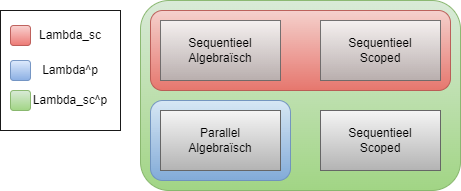
\includegraphics[width=\textwidth]{Media/scope.png}
    \caption{Scope van de verschillende calculi vermeld in deze thesis}
    \label{fig:motiv}
\end{figure}

De primaire motivatie voor de ontwikkeling van de calculus is het ontbreken van een calculus die zowel parallelle als sequentiële uitvoering van zowel algebraïsche als scoped effecten in de literatuur. De $\lambda_{sc}$-calculus \cite{Bosman2022} ondersteunt sequentiële uitvoering van algebraïsche en scoped effecten. De $\lambda^{p}$-calculus ondersteunt parallelle uitvoering van algebraïsche effecten. Het doel van de $\lambda_{sc}^{p}$-calculus is om deze leemte in de literatuur te vullen en zowel parallelle als sequentiële uitvoering van algebraïsche en scoped effecten mogelijk te maken zoals afgebeeld in Figuur \ref{fig:motiv}. \newline
De manier van parallelle uitvoering is zoals uitgewerkt in de $\lambda^p$-calculus, namelijk het opstellen van een nieuw effect of een nieuwe constructie die een lijst van inputs geeft en eenzelfde computatie in parallel uitvoert voor elke input in de lijst. 

\section{Syntaxis}
De syntaxis van de $\lambda^p$-calculus verdeelt de termen in expressies in handlers terwijl die van de $\lambda_{sc}$-calculus de termen verdeelt in waarden en computaties. De gecombineerde calculus houdt de laatste conventie aan en syntactische uitbreidingen voor parallelle uitvoering van de $\lambda^p$-calculus moeten aangepast worden naar deze conventie.

\section{Operationele semantiek}
De $\lambda^p$-calculus modelleert geen complete, klein-stappige operationele semantiek. De semantiek kan in huidige vorm niet ingepast worden in de $\lambda_{sc}$-calculus en zal de introductie en eigen contributie van meerdere nieuwe regels noodzaken om in een klein-stappige operationele semantiek te passen.

\section{Type- en Effect-Systeem}
De $\lambda^p$-calculus heeft geen type- en effect-systeem. De gecombineerde calculus bouwt verder op het systeem van de $\lambda_{sc}$-calculus. De uitbreidingen aan het type- en effect-systeem zullen een significante eigen contributie vormen. 

\section{Metatheorie}
Voor de gecombineerde calculus zal getracht worden de typeveiligheid te bewijzen. De contributie zal voornamelijk bestaan uit het uitbreiden van het bewijs voor \emph{progress} en het bewijs voor \emph{subject reduction} voor de nieuwe set van typerings-regels en semantische regels.



%Omdat parallelle of sequentiële uitvoering een verschil in semantiek geeft en in de effect handler aanpak de semantiek doorgeschoven is naar de handler, gebeurt dit ook in de $\lambda_{sc}^{p}$-calculus voor de semantiek van uitvoeringswijze. Concreet zal elke handler een clausule uitwerken die bepaalt hoe een lijst van computatie met de effecten die de handler behandelt, behandeld worden.

%\subsection{Voorbeeld} 
%\begin{equation} \label{eq:motivEx}
%    \begin{split}
%        \textbf{for}\:(1:2:3:4:5:[\:\:])\:(x.\:\textbf{if}\:x \equiv 2 & \\
%        & \textbf{then}\:\textbf{op}\:throw\:''error''\:(x.\:\textbf{return}\:x);\\
%        & \textbf{else}\:\textbf{op}\:accum\:x\:(x.\:\textbf{return}\:x))\:(x.\:\textbf{return}\:x) \\
%    \end{split}
%\end{equation}

%Het voorbeeld programma in Eq. \ref{eq:motivEx} is een programma dat een accumulatie doet in een string waarbij een functie mapt over een lijst met getallen van 1 tot 5. Dit is een voorbeeld uit \cite{Xie2021} met herwerkte syntaxis. De functie gooit een fout als de input 2 is, anders voegt de functie de input bij het resultaat. Bij sequentiële uitvoering zouden we verwachten dat het programma de executie stopt vanaf het de functie met input 2 behandelt. Het resultaat van de accumulatie is dan "1". Bij parallelle afhandeling gaat de exception bij input 2 geen effect kunnen hebben op de andere accumulaties die parallel gebeuren en zal het resultaat "1345" zijn. Deze verschillende semantiek zou kunnen bekomen worden door 2 verschillende handlers te maken die het exception effect afhandelen waarbij de ene werkt op de sequentiële wijze en de andere op de parallelle wijze.

%Een hoofdstuk behandelt een samenhangend geheel dat min of meer op zichzelf
%staat. Het is dan ook logisch dat het begint met een inleiding, namelijk
%het gedeelte van de tekst dat je nu aan het lezen bent.

%\section{Eerste onderwerp in dit hoofdstuk}
%De inleidende informatie van dit onderwerp.

%\subsection{Een item}
%De bijbehorende tekst. Denk eraan om de paragrafen lang genoeg te maken en
%de zinnen niet te lang.

%Een paragraaf omvat een gedachtengang en bevat dus steeds een paar zinnen.
%Een paragraaf die maar \'e\'en lijn lang is, is dus uit den boze.

%\section{Tweede onderwerp in dit hoofdstuk}
%Er zijn in een hoofdstuk verschillende onderwerpen. We zullen nu
%veronderstellen dat dit het laatste onderwerp is.

%\section{Besluit van dit hoofdstuk}
%Als je in dit hoofdstuk tot belangrijke resultaten of besluiten gekomen
%bent, dan is het ook logisch om het hoofdstuk af te ronden met een
%overzicht ervan. Voor hoofdstukken zoals de inleiding en het
%literatuuroverzicht is dit niet strikt nodig.

%%% Local Variables: 
%%% mode: latex
%%% TeX-master: "masterproef"
%%% End: 

\chapter{Syntaxis}
\label{hoofdstuk:syntaxis}


Dit hoofdstuk bespreekt de syntaxis voor de gecombineerde $\lambda_{sc}^p$-calculus. Tabel \ref{fig:syntaxisNodig} stelt de syntaxis voor met de \emph{nodige uitbreidingen} op de $\lambda_{sc}$-calculus gemarkeerd. 
% De belangrijkste toevoeging is de \textbf{for} clausule in de handler. Bijhorend is een lijst-structuur voor waarden en een lijst-structuur voor computaties. 
Merk op dat de calculus \emph{geen nieuwe effect operatie} introduceert. Sectie \ref{sec:SyntaxFor} bespreekt de reden hiervoor. \newline
Tabel \ref{fig:syntaxisHandig} toont \emph{handige uitbreidingen} om de evaluatie van meer programma's mogelijk te maken. Deze tabel beschrijft een \textbf{let rec} constructie om \emph{recursieve functie evaluatie} mogelijk te maken, een \textbf{if} \emph{conditionele constructie} en enkele hulp-functies om \emph{paar- en lijst-manipulatie} toe te laten. Deze toevoegingen zijn niet essentieel om een minimaal werkende calculus te bekomen maar wel nodig om de voorbeelden te kunnen evalueren. De volgende secties bespreken de verschillende toegevoegde syntactische elementen.

\section{For clausule}
\label{sec:SyntaxFor}
%De \textbf{for} clausule modelleert parallelle behandeling in de calculus. 
Het doel van deze calculus is om zoals in de $\lambda^p$-calculus uitgaande van een parallelle pure \emph{for each} functie parallelle, gebruiker-gedefinieerde parallelle effecten te modelleren\cite{Xie2021}. De $\lambda^p$-calculus gebruikt hiervoor een \textbf{for} clausule in de vorm ''$\textbf{for} \ x : n. \ e$'' om zowel de pure \emph{for each} te presenteren als de \textbf{for} clausule als effect operatie.
\begin{table}[h]
    \centering
    \begin{tabular}{c c c c c c}
        $\lambda^p$-calculus: & \textbf{for} &  & x : n. & e &  (impliciete k) \\
        $\lambda_{sc}$-calculus: & \textbf{sc} & $l^{sc}$ & x & p & k \\  
        & sleutelwoord & label & argument & computatie in scope & continuatie \\
    \end{tabular}
    \caption{Syntaxis vergelijking tussen \textbf{for} in $\lambda^p$ en \textbf{sc} in $\lambda_{sc}$}
    \label{tab:synForSc}
\end{table}
%De \textbf{for} clausule die deze syntaxis aanlevert, bestaat uit het sleutelwoord \textbf{for}, gevolgd door een for-label,  een lijst van waarden, gevolgd door een functie $(y. \ c_{1})$, gevolgd door de resumptie $(z. \  c_{2})$ die de continuatie van het programma bevat. 
Merk op dat de syntaxis van de \textbf{for} clausule sterk gelijkt op die van de \textbf{sc} clausule, met uitzondering van het missen van een label omdat in de $\lambda^p$-calculus slechts \'e\'en parallel effect per programma kan gedefinieerd worden en dat de continuatie niet expliciet is voor het \textbf{for}-statement.
%deze niet als \'e\'en clausule kan beschouwd worden omdat de semantiek zal verschillen. 
%De syntaxis lijkt sterk op de syntaxis uit de $\lambda^p$-calculus met de uitzondering van het toegevoegde label. 
Het label laat toe om meerdere verschillende parallelle/scoped effecten binnen hetzelfde programma te evalueren. \newline 
Deze thesis argumenteert dat de parallel niet stopt bij de syntaxis maar \emph{volledig door te trekken is}.
 %De standaard \textbf{for} behandeling (om een parallelle \emph{for each} constructie te benaderen) zou zijn om de functie, in parallel, op elke waarde in de lijst toe te passen en het resultaat als input van de continuatie te gebruiken. Aangezien de calculus een effect handler aanpak voorstelt, is dat slechts een mogelijke implementatie van de handler. De handler bepaalt hoe de \textbf{for} constructie te behandelen. Aangezien deze computatie nieuwe \textbf{for} constructies kan introduceren, is het raadzaam om elk programma met \textbf{for} constructies als buitenste handler te behandelen door een pure handler om eventuele overgebleven \textbf{for} constructies puur af te handelen.
 %De \textbf{for} clausule heeft in tegenstelling tot de \textbf{op} of \textbf{sc} clausule geen label omdat deze clausule geen specifiek effect voorsteld maar een generieke \textbf{for-each} constructie over een lijst. 

%\begin{equation}
%    \textbf{for}\quad (input_1:input_2:input_3:[\:\:]) \quad (input.\:\textbf{effect}\:input) \quad(result.\:\textbf{rest})
%\end{equation}


%\begin{equation}
%    \begin{split}
%    & \textbf{hPure} = \textbf{handler} \\
%    & \{ \\
%    & \qquad ... \\
%    & \qquad    \textbf{for}\:lst\:p\:k \rightarrow \textbf{do}\:res \leftarrow map\:p\:lst \\
%    &  \qquad \qquad \qquad \qquad k\:res \\
%    & \} 
%\end{split}  
%\end{equation}

\begin{table}
    \centering
    \begin{tabular}{|r c l r|}
    \hline 
         waarden $v$ & $::=$ & $() \ \ | \ \ (v_{1}, \ v_{2} ) \ \ | \ \ x \ \ | \ \ \lambda x . \ c \ \ | \ \ h$ & \\
         & $|$ & \hl{lstV[A]} & \\
         handlers $h$ & $::=$ & $\textbf{handler} \ \{ \ \ \textbf{return} \ x \mapsto c_{r}$ & return clausule\\
         & & $\qquad \qquad \quad , \ oprs$ & effect  clausules \\
         & & $\qquad \qquad \quad , \ \textbf{fwd} \ f \ p \ k \mapsto c_{f} \}$ & forwarding clausule \\
         \hl{lijst waarden $lstV[A]$} & $::=$ & \hl{$nilV[A]\  \  | \  \  consV[A] \ 
 v_1 \  v_2$} & \hl{lijst van waarden}\\
          effect clausules $oprs$ & $::=$ & . & \\ 
          & $|$ & $\textbf{op} \ l^{op} \ x \ k \mapsto c, \ oprs$ & algebraïsch effect clausule\\
           & $|$ & $\textbf{sc} \ l^{sc} \ x \ p \ k \mapsto c, \ oprs$ & scoped effect clausule\\
        % & $|$ & \hl{$\textbf{for}\  l^{for} \  x \  p \  k \mapsto c, \  oprs$} & \hl{for effect clausule} \\
         computaties $c$ & $::=$ & $\textbf{return} \ v$ & return waarde \\
          & $|$ & $\textbf{op} \ l^{op} \ v \ (y. \ c)$ & algebraïsch effect \\
          & $|$ & $\textbf{sc} \ l^{sc} \ v \ (y. \ c_{1}) \ (z. \ c_{2})$ & scoped effect \\
          % & $|$ & \hl{$\textbf{for} \ l^{for} \ v \ (y. \ c_{1}) \ (z. \ c_{2})$} & \hl{for effect} \\
          & $|$ & $v \star c$ & behandeling \\
          & $|$ & $\textbf{do} \ x \leftarrow c_{1}; \ c_{2}$ & do clausule \\
          & $|$ & $v_{1} \ v_{2}$ & applicatie \\
          & $|$ & $\textbf{let} \ x = v \ \textbf{in} \ c$ & let \\
          & $|$ & \hl{\textbf{map} \ $v_1$ \ $v_2$} & \hl{map over lstv} \\
          & $|$ & \hl{$lstC[A]$} & \hl{lijst computaties} \\
          \hl{lijst computaties $lstC[A]$} & $::=$ & \hl{$nilC[A] \ 
 \  | \  \  consC[A] \  c_1 \  c_2$} & \hl{lijst computaties}\\
         waarde types $A, \ B, \ M$ & $::=$ & $() \ \ | \ \ (A, \ B) \ \ | \ \ A \rightarrow \underline{C} \ \ | \ \ \underline{C} \Rightarrow \underline{D}$ & \\
         & $|$ & $\alpha$ & type variabele \\
         & $|$ & $\lambda \ \alpha . \ A$ & type operator abstractie \\
         & $|$ & $M \ A$ & type applicatie \\
         & $|$ & \hl{ListV A} & \hl{lijst waarden}\\
         type schemas $\sigma$ & $::=$ & $A \ \ | \ \ \forall \ \mu . \ \sigma \ \ | \ \ \forall \ \alpha . \ \sigma $ & \\
         computatie types $\underline{C}, \ \underline{D}$ & $::=$ & $A ! \langle E \rangle $ & \\
         & $|$ & \hl{ListC $\underline{C}$} & \hl{lijst computaties}\\
         effect type rows $E, \: F$ & $::=$ & $ . \ \ | \ \ \mu \ \ | \ \ l ; \ E$ & \\
         %kinds $K$ & $::=$ & $* \: \: | \: \: K \rightarrow K$ & \\
         signatuur contexten $\Sigma$ & $::=$ & $ . $ & \\
         & $|$ & $\Sigma , \ l^{op} : A_{op} \rightarrowtriangle B_{op}$ & \\
         & $|$ & $\Sigma , \ l^{sc} : A_{sc} \rightarrowtriangle B_{sc}$ & \\
         % & $|$ & \hl{$\Sigma , \ l^{for} : A_{for} \rightarrowtriangle B_{for}$} & \\
         type contexten $\Gamma$ & $::=$ & $. \: \: | \:\: \Gamma, \: x \: : \: A \: \: | \: \: \Gamma , \: \mu \: \: | \: \: \Gamma, \: \alpha $ & \\
    \hline
    \end{tabular}
    \caption{$\lambda_{sc}^{p}$ Syntaxis met uitbreidingen gemarkeerd}
    \label{fig:syntaxisNodig}
\end{table}


\begin{table}
    \centering
    \begin{tabular}{|r c l r|}
    \hline 
        & & & \\
        waarden $v$ & $::=$ & \hl{true | false} & \hl{booleans} \\
        & & & \\
         computaties $c$ & $::=$ & \hl{$\textbf{let rec} \: f \: = \: c_{1} \: \textbf{in} \: c_{2}$} & \hl{let rec} \\
         & $|$ & \hl{\textbf{if} v \textbf{then} $c_1$ \textbf{else} $c_2$} & \hl {conditie} \\
          & $|$ & \hl{\textbf{headV[A]} \ v} & \hl{head lstv} \\
          & $|$ & \hl{\textbf{tailV[A]} \ v} & \hl{tail lstv} \\
          & $|$ & \hl{\textbf{emptyV[A]} \ v} & \hl{test lege lstv} \\
          & $|$ & \hl{\textbf{headC[A]} \ c} & \hl{head lstc} \\
          & $|$ & \hl{\textbf{tailC[A]} \ c} & \hl{tail lstc} \\
          & $|$ & \hl{\textbf{emptyC[A]} \ c} & \hl{test lege lstc} \\
          & $|$ & \hl{\textbf{fst}\:v} & \hl{first paar} \\
          & $|$ & \hl{\textbf{snd}\:v} & \hl{second paar} \\
          & & & \\
          waarde types $A, \: B, \: M$ & $::=$ & \hl{Bool} & \hl{boolean} \\ 
         & & & \\
    \hline
    \end{tabular}
    \caption{Uitbreidingen op de $\lambda_{sc}^{p}$ Syntaxis om de calculus meer bruikbaar te maken}
    \label{fig:syntaxisHandig}
\end{table}

\section{Lijst-structuur}
De calculus heeft nood aan een manier om een pure parallelle for each functie te definiëren. De minimale vereiste om computaties in parallel uit te voeren is een samengestelde datastructuur waarop een parallelle iterator kan gedefinieerd worden om een functie toe te passen op de verschillende inputwaarden.
%samengestelde data-structuur in de calculus die de verschillende computaties die de machine parallel uitvoert bijhoudt. 
Deze calculus gebruikt een lijst-structuur maar in principe is elke lineaire datastructuur mogelijk. \newline
%op elke lineaire datastructuur. \newline
%aangezien op elk van deze het mogelijk is (maar niet noodzakelijk efficiënt) een head, tail en empty functie te implementeren. 
%Een voorbeeld van een lijst van computaties is: 
%\begin{equation} \label{eq:listEx}
%    \begin{split}
%    (39 + 49):(29 + 74):(100 + 61):(41 + 56):(97 + 67):[\:\:] \\
%    \leadsto 88:103:161:97:164:[\:\:]
%    \end{split}
%\end{equation} 
%De reductie in dit voorbeeld kan parallel gebeuren voor elk element in de lijst. \newline
Aangezien de $\lambda_{sc}$-calculus syntaxis een strikte scheiding hanteert tussen waarden en termen ligt het voor de hand dat de $\lambda_{sc}^{p}$-calculus eveneens strikt onderscheid maakt tussen \emph{lijsten van waarden} en \emph{lijsten van computaties}. \newline
De syntaxis neemt inspiratie van de syntaxis voor lijsten beschreven in Hoofdstuk 11.12 in TAPL\cite{Pierce2002}.

\subsection{Lijst van waarden}
Een lijst van waarden is zelf een waarde. De syntaxis is intuïtief, de lijst is een lege lijst ($nilV[A]$) van een bepaald type A of een compositie van een waarde en een lijst ($consV[A] \  v_1 \ 
 v_2$), de waarde met type A en de lijst met type ListV van A. Het type-systeem in \Cref{hoofdstuk:typesysteem} controleert de vereiste dat de waarden het juiste type bezitten. De lijst van waarden voegt het waarde type $ListV \ A$ toe.

\subsection{Lijst van computaties}
%Een lijst van compuaties is een computatie, dit omdat de elementen in de lijst kunnen reduceren en semantische regels geïntroduceerd worden in Sectie \ref{hoofdstuk:semantiek} om een lijst te reduceren naar een lijst van normaalwaarden. Hiervoor moet de lijst zelf een computatie zijn omdat een reductie in de $\lambda_{sc}^{p}$-calculus een computatie naar een andere computatie mapt. 
De syntaxis voor een lijst van computaties is intuïtief en analoog aan de lijst van waarden. De lijst is een lege lijst ($nilC[A]$) van een bepaald type A of een compositie van een computatie en een lijst ($consC[A] \  c_1 \ 
 c_2$), de computatie met type A en de lijst met type ListC van $\underline{C}$. Het type-systeem in \Cref{hoofdstuk:typesysteem} controleert de vereiste dat de computaties het juiste type bezitten. De lijst van computaties voegt het computatie type $ListC \ \underline{C}$ toe.

\subsection{Lijst-manipulatie functies}
Om voorbeelden uit te werken heeft de lijst-structuur een \textbf{head}, \textbf{tail} en \textbf{empty} functie nodig om elementen uit de lijst te halen en na te kijken of de lijst leeg is. Deze minimale implementatie is aanwezig in de syntaxis door de \emph{\textbf{headV[A]} v, \textbf{tailV[A]} v, \textbf{emptyV[A]} v, \textbf{headC[A]} c, \textbf{tailC[A]} c en \textbf{emptyC[A]} c} computaties. De volgende voorbeelden illustereren kort de syntaxis en semantiek van deze functies. De calculus is in de voorbeelden impliciet uitgebreid met een $Int$ basis-type.

\begin{equation}
    \begin{split}
        & \textbf{headV[Int]}\:(consV[Int] \  5 \  consV[Int] \  3 \  consV[Int] \  8 \  nilV[Int]) \\
        & \leadsto \textbf{return}\:5
    \end{split}
\end{equation}
Veronderstel in de volgende voorbeelden dat de calculus is uitgebreid met een \textbf{double} computatie die een $Int$ verdubbelt.

\begin{equation}
    \begin{split}
        & \textbf{headC[Int]}\:(consC[Int] \  (\textbf{double} \ 5) \   consC[Int] \ 
 (\textbf{double} \ 3) \  nilC[Int]) \\
        & \leadsto \textbf{return}\:(\textbf{double}\:5)
    \end{split}
\end{equation}

\begin{equation}
    \begin{split}
        & \textbf{tailV[Int]} \ (consV[Int] \ 5 \ consV[Int] \  3 \  consV[Int] \  8 \  nilV[Int]) \\
        & \leadsto \textbf{return} \  (consV[Int] \  3 \  consV[Int] \  8 \  nilV[Int])
    \end{split}
\end{equation}

\begin{equation}
    \begin{split}
        & \textbf{tailC[Int]} \ (consC[Int] \  (\textbf{double}\:5) \ 
 consC[Int] \  (\textbf{double}\:3) \ nilC[Int]) \\
        & \leadsto \textbf{return}\:(consC[Int] \  (\textbf{double}\:3) \ nilC[Int) 
    \end{split}
\end{equation}

\begin{equation}
    \begin{split}
        & \textbf{emptyV[Int]}\:(consV[Int] \ 5 \  nilV[Int]) \\
        & \leadsto \textbf{return}\:false
    \end{split}
\end{equation}

\begin{equation}
    \begin{split}
        & \textbf{emptyC[Int]} \ (consC[Int] \ (\textbf{double}\:5) \ nilC[Int]) \\
        & \leadsto \textbf{return}\:false
    \end{split}
\end{equation}


\begin{equation}
    \begin{split}
        & \textbf{emptyV[Int]} \ nilV[Int] \\
        & \leadsto \textbf{return} \ true
    \end{split}
\end{equation}

\begin{equation}
    \begin{split}
        & \textbf{emptyC[Int]} \ nilC[Int] \\
        & \leadsto \textbf{return} \ strue
    \end{split}
\end{equation}

\subsection{Map functie}
De \textbf{map} constructie modelleert een functie die een lijst van waarden omvormt naar een lijst van computaties met als argument een lambda-functie om toe te passen op de lijst van waarden. Hieronder een demonstratie doormiddel van een simpel voorbeeld en het uiteindelijke resultaat na evaluatie.

\begin{equation}
    \begin{split}
        & \textbf{map}\:(\lambda x . \ x+1)\:(consV[Int] \ 5 \ consV[Int] \  3 \  consV[Int] \ 8 \  nilV[Int]) \\
        & \leadsto * \quad \textbf{return} \  (consV[Int] \ 6 \ consV[Int] \  4 \  consV[Int] \ 9 \  nilV[Int])
    \end{split}
\end{equation}
Het doel van deze constructie is om de \emph{parallelle constructie} te vormen die een lijst van computaties vormt die allen in parallel geëvalueerd worden. De calculus wijkt hier af van de $\lambda^p$-calculus aangezien door de scheiding te maken waar in $\lambda^{p}$ de \textbf{for} clausule beide rollen opneemt. Enerzijds de effect operatie zoals in de \textbf{E-Traverse} regel en anderzijds de pure, parallelle for each als in de \textbf{E-Parallel} regel. \newline 
Een voordeel van de expliciete scheiding is dat deze calculus ook eenvoudig gebruik kan maken van pure parallelle for each door de \textbf{map} constructie.

\section{Recursieve let}
De \textbf{let rec} constrcutie laat toe om recursieve functies te implementeren in de calculus. De syntaxis is voornamelijk gebaseerd op de syntaxis voor \textbf{let rec} beschreven in hoofdstuk twee van het boek "Principles of Programming Languages" \cite{Palmer2009} en les 11 van CS6110 aan de Cornell-universiteit \cite{Sampson2018} maar wordt op soortgelijke manier voorgesteld in TAPL \cite{Pierce2002} in Sectie 11.11. \newline 
%Voor simpliciteit is gekozen om slechts 1 recursieve functie toe te laten in tegenstelling tot implementaties die een lijst van recursieve functies toelaten. Dit in referentie naar de syntaxis van \textbf{letrec}, $\textbf{letrec} \ f = c_1 \ in \ c_2$ waarbij de $c_1$ ook een lijst. omdat deze implementatie de semantische regels vereenvoudigt en voldoende expressief is om de gewenste voorbeelden uit te werken. \newline 
Recursieve functies zijn nodig om enkele functies te definiëren die handig zijn om interessante voorbeelden uit te worken zoals bijvoorbeeld een implementatie van foldr:

\begin{equation} \label{eq: sumEx}
    \begin{split}
        \textbf{let\:rec}\:foldr\:= &\:l\:op\:mempty.\: \\
        & \textbf{do}\:n\leftarrow \textbf{empty}\:l; \\
        & \textbf{if}\:n\:\textbf{then}\:\textbf{return}\:mempty \\
        & \textbf{else} \\
        & \qquad \textbf{do}\:h \leftarrow \textbf{head}\:l;\\
        & \qquad \textbf{do}\:t \leftarrow \textbf{tail}\:l; \\
        & \qquad \textbf{do}\:y \leftarrow \textbf{foldr}\:t\:op\:mempty    ; \\
        & \qquad \textbf{return}\:(op\:h\:y)\:\textbf{in} \\
        & \qquad \qquad \textbf{foldr}\:(consV[Int] \  1 \  consV[Int] \ 2 \ nilV[Int])\:(+)\:0;\\
    \end{split}
\end{equation}

Dit voorbeeld programma telt de waarden in de lijst [1,2] op tot 3.

\section{Booleans}
Een handige praktische toevoeging aan de calculus is om booleans toe te voegen als basis type. Deze uitbreiding laat vervolgens een extensie met condities die meer expressieve voorbeelden toelaten.

\begin{equation}
    true
\end{equation}

\begin{equation}
    false
\end{equation}

\section{Conditie}
Een simpele conditie om de controlestroom van programma's te bepalen op basis van een test.

\begin{equation}
    \begin{split}
        & \textbf{if}\  true \  \textbf{then} \  \textbf{return} \  0 \  \textbf{else} \  \textbf{return} \  1 \\
        & \leadsto \textbf{return}\  0
    \end{split}
\end{equation}

\begin{equation}
    \begin{split}
        & \textbf{if}\  false \  \textbf{then} \  \textbf{return} \  0 \  \textbf{else} \  \textbf{return} \  1 \\
        & \leadsto \textbf{return}\  1
    \end{split}
\end{equation}





%%% Local Variables: 
%%% mode: latex
%%% TeX-master: "masterproef"
%%% End: 

\chapter{Operationele Semantiek}
\label{hoofdstuk:semantiek}
\begin{table}
    \centering
    \begin{tabular}{|l|}
        \hline
        % top
        \\
        % header
         \begin{tabular} {l r}
              \begin{tabular}{|l|}
              \hline
                     $c \leadsto c'$ \\
                \hline
              \end{tabular} & Computatie reductie \\
         \end{tabular} \\
         % rules
          \begin{tabular}{c}
            $\inference{}{(\lambda x.\:c)\:v \leadsto c\:[\:v\:/\:x\:]}[E-AppAbs] \qquad \inference{}{\textbf{let}\:x\: = \: v \: \textbf{in} \:c \leadsto c\:[\:v\:/\:x\:]}[E-Let]$ \\ 
            \\
            $\inference{}{\textbf{let\:rec}\:f\:=\:c_{1}\:\textbf{in}\:c_{2} \leadsto c_{2}\:[c_{1}\:[(\textbf{let\:rec}\:f\:=\:c_{1}\:\textbf{in}\:f)\:/\:f]\:/\:f]}[\hl{E-Letrec}]$ \\
            \\
            $\inference{c_{1} \leadsto c_{1}'}{\textbf{do}\:x \leftarrow c_{1}\:;\:c_{2} \leadsto \textbf{do}\:x \leadsto c_{1}'\:;\:c_{2}}[E-Do] \qquad \inference{}{\textbf{do}\:x \leftarrow \textbf{return}\:v\:;\:c_{2} \leadsto c_{2}\:[\:v\:/\:x\:]}[E-DoRet]$ \\
            \\
            $\inference{}{\textbf{do}\:x \leftarrow \textbf{op}\:l\:v\:(y.\:c_{1})\:;\:c_{2} \leadsto \textbf{op}\:l\:v\:(y.\: \textbf{do} \: x \leftarrow c_{1}\:;\:c_{2})}[E-DoOp]$ \\
            \\
            $\inference{}{\textbf{do}\:x \leftarrow \textbf{sc} \:l\:v\:(y.\:c_{1})\:(z.\:c_{2}) \: ;\: c_{3} \leadsto \textbf{sc} \:l\:v\:(y.\:c_{1})\:(z.\: \textbf{do} \: x \leftarrow c_{2} \: ;\: c_{3})}[E-DoSc]$ \\
            \\
            $\inference{}{\textbf{do}\:x \leftarrow \textbf{for}\:lstv\:(y.\:c_{1}) (z.\:c{2});\:c_{3} \leadsto \textbf{for}\:lstv\:(y.\:c_{1})\:(z.\:\textbf{do}\:x \leftarrow c_{2};\:c_{3})}[\hl{E-DoFor}]$ \\
            \\
            $\inference{c \leadsto c'}{h \star c \leadsto h \star c'}[E-Hand] \qquad \inference{(\textbf{return}\:x \mapsto c_{r}) \in h}{h \star \textbf{return} \: v \leadsto c_{r} \:[\:v\:/\:x\:]}[E-HandRet]$ \\
            \\
            $\inference{(\textbf{op}\:l\:x\:k \mapsto c) \in h}{h \star \textbf{op}\:l\:v\:(y.\:c_{1}) \leadsto c\:[\:v\:/\:x,\:(\lambda y.\:h \star c_{1}) \: / \: k]}[E-HandOp]$ \\
            \\
            $\inference{(\textbf{op}\:l\:\_\:\_) \notin h}{h \star \textbf{op}\:l\:v\:(y.\:c_{1}) \leadsto \textbf{op}\:l\:v\:(y.\: h \star c_{1})}[E-FwdOp]$ \\
            \\
            $\inference{(\textbf{sc}\:l\:x\:p\:k \mapsto c) \in h}{h \star \textbf{sc}\:l\:v\:(y.\:c_{1})\:(z.\:c_{2}) \leadsto c\:[\:v\:/\:x,\:(\lambda \: y. \: h \star\:c_{1}) \: / \: p, (\lambda z. \: h \star c_{2}) \:/\:k\:]}[E-HandSc]$ \\
            \\
            $\inference{(\textbf{sc}\:l\:\_\:\_\:\_) \notin h \\ (\textbf{fwd}\:f\:p\:k \mapsto c_{f}) \in h \qquad g\:=\:\lambda(p',\:k')\:.\:\textbf{sc}\:l\:v\:(y.\:p'\:y)\:(z.\:k'\:z)}{h \star \textbf{sc}\:l\:v\:(y.\:c_{1})\:(z.\:c_{2}) \leadsto c_{f}\:[\:(\lambda\:y.\:h \star c_{1})\:/\:p,\:(\lambda z.\: h \star c_{2})\:/\:k,\:g\:/\:f]}[E-FwdSc]$\\
            \\
            $\inference{(\textbf{for}\:lstv_{1}\:p\:k \mapsto c_{for}) \in h}{h \star \textbf{for}\:lstv_{2}\:(y.\:c_{1})\:(z.\:c_{2}) \leadsto c_{for}[lstv_{2}\:/\:lstv_{1},\:(y.\:h \star c_{1})\:/\:p, (z.\:h \star c_{2})\:/\:k]}[\hl{E-HandFor}]$\\
            \\
            $\inference{(\textbf{for}\:\_\:\_\:\_ \notin h)}{h \star \textbf{for}\:lstv\:(y.\:c_1)\:(z.\:c_2) \leadsto \textbf{for}\:lstv\:(y.\:h \star c_1)\:(z.\: h \star c_2)}[\hl{E-FwdFor}]$ 
          \end{tabular} \\
          % bottom
          \\
        \hline
    \end{tabular}
    \caption{Operationele semantiek van $\lambda_{sc}^{p}$}
    \label{fig:semantiek}
\end{table}

\begin{table}
    \centering
    \begin{tabular}{|l|}
        \hline
        \\
        \begin{tabular} {l r}
              \begin{tabular}{|l|}
              \hline
                     $c \leadsto c'$ \\
                \hline
              \end{tabular} & Computatie reductie \\
         \end{tabular} \\
         \begin{tabular}{c}
          $\inference{}{\textbf{map}\:f\:(v_{1}:v_{2}:\:...\::v_{n}:[\:\:]) \leadsto
          ((f\:v_{1}):(f\:v_{2}):\:...\::(f\:v_{n}):[\:\:])}[\hl{E-Map}]$\\
          \\
          $\inference{1 \leq i \leq n \qquad c_i \leadsto c_i'}{(c_1:...:c_i:...:c_{n}:[\:\:]) \leadsto (c_1:...:c_i':...:c_{n}:[\:\:])}[\hl{E-ParList}]$\\
          \\
          $\inference{}{((\textbf{return}\:v_1):(\textbf{return}\:v_2):...:(\textbf{return}\:v_n):[\:\:]) \leadsto \textbf{return}\:(v_1:v_2:...:v_n:[\:\:])}[\hl{E-ListRet}]$ \\
          \\
          $\inference{}{\textbf{head}\:(v_1:lstv) \leadsto \textbf{return}\:v_1}[\hl{E-HeadLstv}] \qquad \inference{}{\textbf{head}\:(c_1:lstc) \leadsto \textbf{return}\:c_1}[\hl{E-HeadLstc}]$ \\
          \\
        $\inference{}{\textbf{tail}\:(v_1:lstv) \leadsto \textbf{return}\:lstv}[\hl{E-TailLstv}] \qquad \inference{}{\textbf{tail}\:(c_1:lstc) \leadsto \textbf{return}\:lstc}[\hl{E-TailLstc}]$ \\
        \\
        $\inference{}{\textbf{empty}\:[\:\:] \leadsto \textbf{return}\:true}[\hl{E-EmptyTrue}]$ \\
        \\
        $\inference{}{\textbf{empty}\:(v:lstv) \leadsto \textbf{return}\:false}[\hl{E-EmptyLstvFalse}]$\\ 
        \\
        $\inference{}{\textbf{empty}\:(c:lstc) \leadsto \textbf{return}\:false}[\hl{E-EmptyLstcFalse}]$ \\
        \\
        $\inference{}{\textbf{fst}\:(v_1,\:v_2) \leadsto \textbf{return}\:v_1}[\hl{E-First}] \qquad \inference{}{\textbf{snd}\:(v_1,\:v_2) \leadsto \textbf{return}\:v_2}[\hl{E-Second}]$ \\
        \\
        $\inference{c_1 \leadsto c_1'}{\textbf{if}\:c_1\:\textbf{then}\:c_2\:\textbf{else}\:c_3 \leadsto \textbf{if}\:c_1'\:\textbf{then}\:c_2\:\textbf{else}\:c_3}[\hl{E-If}]$\\
        \\
        $\inference{}{\textbf{if}\:true\:\textbf{then}\:c_1\:\textbf{else}\:c_2 \leadsto c_1}[\hl{E-IfTrue}]$\\
        \\
        $\inference{}{\textbf{if}\:false\:\textbf{then}\:c_1\:\textbf{else}\:c_2 \leadsto c_2}[\hl{E-IfFalse}]$\\
        \\
         \end{tabular}
         \\
          \hline
    \end{tabular}
    \caption{Operationele semantiek van $\lambda_{sc}^{p}$, lijst- en hulp-functies}
    \label{tab:opSemLst}
\end{table}

Tabellen \ref{fig:semantiek} en \ref{tab:opSemLst} toont de operationele semantiek voor de $\lambda_{sc}^{p}$-calculus. De toegevoegde regels zijn gemarkeerd. De meest cruciale toevoegingen zijn de regels rond de toevoeging van het nieuwe sleutelwoord \textbf{for}, namelijk \textbf{E-DoFor} voor het aaneenrijgen van computaties, \textbf{E-HandFor} voor het behandelen van de \textbf{for}-constructie door de handler die dit behandelt en \textbf{E-FwdFor} voor het forwarden van \textbf{for}. Het inzicht dat dit niet generiek kan gebeuren, is hierbij belangrijk. Gelijkaardige regels waren nodig voor de \textbf{sc} en \textbf{op} sleutelwoorden met dezelfde functies. Verder zijn enkele toevoegingen gedaan om recursieve functie-behandeling mogelijk te maken (\textbf{E-Letrec}) en lijst- en andere hulp-functies (Tabel \ref{tab:opSemLst}) expliciet toe te voegen. De bestaande regels uit de $\lambda_sc$-calculus \cite{Bosman2022} blijven onveranderd.

\section{Letrec: Recursieve functies}
De \textbf{let rec} constructie biedt de mogelijk om recursieve functies te definiëren in de calculus. De clausule bestaat uit het \textbf{let rec} sleutelwoord gevolgd door een variabele-naam $f$ gevolgd door een computatie $c_{1}$ waar de variabele $f$ in kan voorkomen gevolgd door het sleutelwoord \textbf{in} gevolgd door de computatie waarin de variable $f$ kan voorkomen. Deze clausule wordt gereduceerd naar $c_{2}$ met f in $c_{2}$ vervangen door $c_{1}$ met $f$ vervangen door $\textbf{let\:rec}\:=\:c_{1}\:\textbf{in}\:f$. \textbf{E-Letrec} is een aangepaste versie van de regel beschreven in hoofdstuk twee van het boek "Principles of Programming Languages" \cite{Palmer2009}.

\section{For clausule}
Het \textbf{for} sleutelwoord laat toe om een computatie te mappen over een lijst van waarden. De gewenste semantiek om computaties met eventueel effecten te mappen over een lijst van waarden is niet mogelijk via een klassieke map functie omdat de computatie in dit geval niet puur is en alle relevante handlers niet noodzakelijk binnen de computatie zitten. Het gevolg is dat een klassieke map aanpak vastloopt op een normaalvorm (\textbf{return, op} of \textbf{sc}). Om een correcte semantiek voor het \textbf{for} sleutelwoord te bekomen zijn drie semantische regels nodig.

\subsection{E-DoFor}
\textbf{E-DoFor} laat toe om een \textbf{do} statement door te schuiven naar de continuatie van de \textbf{for} constructie en tegelijk de computatie na de \textbf{for} constructie binnen de continuatie te brengen. Deze regel is nodig om programma's correct aan elkaar te rijgen rond het gebruik van \textbf{for} constructies en is zeer gelijkaardig aan \textbf{E-DoRet}, \textbf{E-DoOp} en \textbf{E-DoSc}.

\subsection{E-HandFor}
\textbf{E-HandFor} laat toe om een \textbf{for} constructie te behandelen door een handler. De \textbf{for} constructie wordt hierbij vervangen door de $c_{for}$ computatie in de handler waarbij de handler eveneens naar binnen geschoven wordt in de te mappen functie en de continuatie. Elke handler kan de clausule implementeren of laten forwarden (\textbf{E-FwdFor}, \Cref{sec:fwdfor}). Aangezien deze behandeling nieuwe \textbf{for} constructies kan introduceren is het raadzaam om vooraan het programma een handler te implementeren die overgebleven pure \textbf{for} constructies afhandelt. De implementatie van deze clausule specifieert of de handler de constructie in parallel of sequentieel afhandelt.

\subsection{E-FwdFor} \label{sec:fwdfor}
\textbf{E-FwdFor} behandelt de forwarding voor het geval dat de \textbf{for} clausule niet door de handler geïmplementeerd wordt. De functie van de forwarding is tweevoudig. Deze regel schuift de handler binnen de computatie die te mappen is en de resumptie.

\section{Lijst- en hulp-functies}
Deze sectie behandelt toevoegingen aan de calculus die nodig zijn voor lijst-manipulatie en hulp-functies die de implementatie van de semantiek van de \textbf{for} clausule vergemakkelijken. 
\subsection{E-Map}
Via deze regel kan in de calculus een lijst van waarden worden omgevormd naar een lijst van computaties met behulp van een computatie $f$. Deze regel is essentieel om deze omvorming te maken. De \textbf{E-ListRet}-regel helpt bij de omvorming in de andere richting. 
\subsection{E-ParList}
\textbf{E-ParList} laat parallelle reductie van elementen in een lijst van computaties toe. De regel stelt dat een element in de lijst dat een stap kan maken, deze stap zet. Merk op dat dit een niet-deterministisch regel is. De voorwaarde om nog een stap te kunnen zetten is dat de computatie niet in normaalvorm is, met andere woorden niet in de vorm:
\begin{equation}
    \textbf{return}\:\_ \:\:|\:\:\textbf{op}\:\:\_\:\_\:\_\:\:|\:\:\textbf{sc}\:\_\:\_\:\_\:\_\:\:|\:\:\textbf{for}\:\_\:\_\:\_\:\_
\end{equation}

\subsection{E-ListRet}
Als een lijst van computaties gereduceerd kan worden naar een lijst van \textbf{return} clausules van waarden, dan kan de lijst vervangen worden door een \textbf{return} clausule van de lijst van waarden. Deze clausule laat, in combinatie met \textbf{E-DoRet}, toe om een lijst van computaties om te vormen naar een lijst van waarden.

\subsection{Lijst-manipulatie}
\textbf{E-HeadLstv}, \textbf{E-HeadLstc}, \textbf{E-TailLstv}, \textbf{E-TailLstc}, \textbf{E-EmptyTrue}, \textbf{E-EmptyLstvFalse} en \textbf{E-EmptyLstcFalse} zijn eenvoudige functies die lijst-manipulatie van lijsten van waarden en lijsten van computaties vergemakkelijken.

\subsection{Paar-manipulatie}
\textbf{E-First} en \textbf{E-Second} laten manipulatie van paren van waarden toe.

\subsection{If constructie}
\textbf{E-If}, \textbf{E-IfTrue} en \textbf{E-IfFalse} implementeren op standaardwijze een \textbf{if} clausule.


%%% Local Variables: 
%%% mode: latex
%%% TeX-master: "masterproef"
%%% End: 

\chapter{Type- en Effect-Systeem}
% TODO: weg For
% TODO: denk over T-For en T-OprFor
% TODO: misschien toch ook handige uitbreidingen typeren? booleans, letrec, condities, ...
% TODO: typering nalezen
\label{hoofdstuk:typesysteem}
Dit hoofdstuk behandelt het type- en effect-systeem van de $\lambda^{p}_{sc}$-calculus. De focus ligt hierbij op de \emph{
toevoegingen} aan het type-systeem van de $\lambda_{sc}$-calculus waar dit systeem op gebaseerd is. Het startpunt waarop dit systeem verderbouwt is beschreven in Sectie \ref{sec:typeScCalc}. In het bijzonder behandelt dit typesysteem de syntaxis zoals beschreven in Figuur \ref{fig:syntaxisNodig}. Aangezien het argument van deze thesis is dat de \emph{parallelle effecten een specifieke vorm van scoped effecten} zijn, zijn de toevoegingen beperkt tot de uitbreidingen voor de lijsten en de \textbf{map} constructie.

\section{Waarde typering}
\begin{table}
    \centering
    \begin{tabular}{|l|}
        \hline
        % top
        \\
        % header
         \begin{tabular} {l r}
              \begin{tabular}{|l|}
              \hline
                     $\Gamma \vdash v\::\:\sigma$ \\
                \hline
              \end{tabular} & Waarde typering \\
         \end{tabular} \\
         % rules
          \begin{tabular}{c}
          \\
            $\inference{(x : \sigma) \in \Gamma}{\Gamma \vdash x : \sigma}[T-Var] \qquad \inference{}{\Gamma \vdash ( \ ) : ( \ )}[T-Unit]$ \\ 
            \\
            $\inference{\Gamma \vdash v_1 : A \qquad \Gamma \vdash v_2 : B}{\Gamma \vdash (v_1 , \ v_2) : (A, \ B)}[T-Pair]$\\
            \\
            $\inference{\Gamma , \ x : A \vdash c : \underline{C}}{\Gamma \vdash \lambda \ x . \ c : A \rightarrow \underline{C}}[T-Abs] \qquad \inference{\Gamma \vdash v : A \qquad A \equiv B}{\Gamma \vdash v : B}[T-EqV]$\\
            \\
            $\inference{\Gamma \vdash v : \forall \ \alpha \ . \ \sigma \qquad \Gamma \vdash A }{\Gamma \vdash v : [ \ A \ / \ \alpha \ ] \ \sigma}[T-Inst] \qquad \inference{\Gamma , \ \alpha \vdash v : \sigma \qquad \alpha \notin \Gamma}{\Gamma \vdash v : \forall \ \alpha . \ \sigma}[T-Gen]$\\
            \\
            $\inference{\Gamma \vdash v : \forall \ \mu . \ \sigma \qquad \Gamma \vdash E}{\Gamma \vdash v : [ \ E \  / \ \mu \ ] \ \sigma}[T-InstEff] \qquad \inference{\Gamma , \ \mu \vdash v : \sigma \qquad \mu \notin \Gamma}{\Gamma \vdash v : \forall \ \mu . \ \sigma}[T-GenEff]$\\
            \\
            $\inference{}{\Gamma \vdash nilV[A] : ListV A}[\hl{T-NilV}] \qquad \inference{\Gamma \vdash v_1 : A \quad \Gamma \vdash c_2 : ListV A}{\Gamma \vdash consV[A] \  v_1 \  v_2 : ListV A}[\hl{T-ConsV}]$ \\
          \end{tabular} \\
          % bottom
          \\
        \hline
    \end{tabular}
    \caption{Waarde typering van $\lambda_{sc}^{p}$}
    \label{fig:typeW}
\end{table}
% Verwijzen naar verschil in syntaxis, enige toevoeging is lijst van waarden... lstv
% 2 nieuwe regels, voor lege lijst en voor lijst op te bouwen
Figuur \ref{fig:typeW} toont de typering voor waarden in de calculus. De toevoegingen tegenover Figuur \ref{fig:typeWaarde} zijn gemarkeerd. Merk op dat aangezien de calculus de syntaxis van waarden enkel uitbreidt met een lijst van waarden zoals aangeduid in Figuur \ref{fig:syntaxisScoped} de enige nieuwe type-regels betrekking hebben tot de typering van lijsten van waarden. De typering voor de lijsten onleent inspiratie van Sectie 11.12 uit TAPL\cite{Pierce2002}. \newline
\textbf{T-NilV} typeert de lege lijst van type A ($NilV[A]$) als een lijst van waarden met type A ($ListV \  A$). \newline
\textbf{T-ConsV} typeert de compositie van een waarde van type A met een bestaande lijst van waarden van type A tot een nieuwe lijst van waarden van type A.

\section{Computatie typering}

\begin{table}
    \centering
    \begin{tabular}{|l|}
        \hline
        % top
        \\
        % header
         \begin{tabular} {l r}
              \begin{tabular}{|l|}
              \hline
                     $\Gamma \vdash c\::\:\underline{C}$ \\
                \hline
              \end{tabular} & Computatie typering \\
         \end{tabular} \\
         % rules
          \begin{tabular}{c}
          \\
            $\inference{\Gamma \vdash v_1 : A \rightarrow \underline{C} \qquad \Gamma \vdash v_2 : A}{\Gamma \vdash v_1 \ v_2 : \underline{C}}[T-App]$ \\
            \\
            $\inference{\Gamma \vdash c_1 : A ! \langle E \rangle \qquad \Gamma , \ x : A \vdash c_2 : B ! \langle E \rangle}{\Gamma \vdash \textbf{do} \ x \leftarrow c_1; \ c_2 : B ! \langle E \rangle}[T-Do]$\\
            \\
            $\inference{\Gamma \vdash c : \underline{C} \qquad \underline{C} \equiv \underline{D}}{\Gamma \vdash c : \underline{D}}[T-EqC] \qquad \inference{\Gamma \vdash v : \sigma \qquad \Gamma , \ x : \sigma \vdash c : \underline{C}}{\Gamma \vdash \textbf{let} \ x = v \ \textbf{in} \ c : \underline{C}}[T-Let]$\\
            \\
            $\inference{\Gamma \vdash v : A \qquad \Gamma \vdash E}{\Gamma \vdash \textbf{return} \ v : A ! \langle E \rangle}[T-Ret] \qquad \inference{\Gamma \vdash v : \forall \ \alpha . \ \alpha ! \langle E \rangle \Rightarrow M \ \alpha ! \langle F \rangle \\ \Gamma \vdash c\::\:A!\langle E \rangle}{\Gamma \vdash v \star c\::\:M\:A!\langle F \rangle}[T-Hand]$\\
            \\
            $\inference{(l^{op} : A_{op} \rightarrowtriangle B_{op}) \in \Sigma \\ \Gamma \vdash v : A_{op} \qquad \Gamma , \ y : B_{op} \vdash c : A ! \langle E \rangle \qquad l^{op} \in E}{\Gamma \vdash \textbf{op} \ l^{op} \ v \ (y . \ c) : A ! \langle E \rangle}[T-Op]$\\
            \\
            $\inference{(l^{sc} : A_sc \rightarrowtriangle B_sc) \in \Sigma \\ \Gamma \vdash v : A_{sc} \qquad \Gamma , \ y : B_{sc} \vdash c_1 : B ! \langle E \rangle \qquad \Gamma , \ z : B \vdash c_2  : A ! \langle E \rangle \qquad l^{sc} \in E}{\Gamma \vdash \textbf{sc} \ l^{sc} \ v \ (y. \ c_1) \ (z. \ c_2) : A ! \langle E \rangle}[T-Sc]$\\
            \\ % TODO: z : B goed of is meer vrijheid nodig?
            %$\inference{(l^{for} : A_{for} \rightarrowtriangle B_{for}) \in \Sigma \\ \Gamma \vdash v : ListV \ A_{for} \qquad
            %\Gamma , \ y : B_{for} \vdash c_1 : B ! \langle E \rangle \qquad \Gamma , \ z : B \vdash c_2 : A!\langle E \rangle \qquad l^{for} \in E }{\Gamma \vdash \textbf{for} \ l^{for} \ v \ (y. \ c_1) \ (z. \ c_2) : A!\langle E \rangle}[\hl{T-For}]$\\
            %\\
            $\inference{}{\Gamma \vdash nilC[\underline{C}] : ListC \ \underline{C}}[\hl{T-NilC}] \qquad \inference{\Gamma \vdash c : \underline{C} \quad \Gamma \vdash lstC[\underline{C}] : \underline{C}}{\Gamma \vdash consC[\underline{C}] \ c \ lstC[\underline{C}] : ListC \ \underline{C}}[\hl{T-ConsC}]$\\
            \\
            $\inference{\Gamma \vdash c_1 : A \rightarrow C \qquad \Gamma \vdash v_2 : ListV \ A}{\textbf{map} \ v_1 \ v_2 : ListC \ \underline{C}}[\hl{T-Map}]$\\
            \\
          \end{tabular} \\
          % bottom
          \\
        \hline
    \end{tabular}
    \caption{Computatie typering van $\lambda_{sc}$}
    \label{fig:typeC}
\end{table}

Figuur \ref{fig:typeC} toont de typering voor computaties in de calculus overgenomen van de $\lambda_{sc}$-calculus met uitbreidingen voor lijsten van computaties. De volgende subsecties bespreken de toegevoegde regels.

%\subsection{T-For}
%Deze subsectie bespreekt de \textbf{T-For} regel die de parallelle effecten typeert. Analaag aan de \textbf{T-Op} en \textbf{T-Sc} regels levert het opzoeken van een het label $l^{for}$ in $\Sigma$ een signatuur $A_{for} \rightarrowtriangle B_{for}$ op. 

\subsection{Lijsten}
De regels \textbf{T-NilC} en \textbf{T-ConsC} die lijsten van computaties typeren zijn gelijkaardig aan de eerder besproken regels \textbf{T-NilV} en \textbf{T-ConsV} maar gegroepeerd onder de Figuur \ref{fig:typeC} aangezien lijsten van computaties zelf computaties zijn in de calculus.

%TODO: meer
\subsection{Map}
De regel \textbf{T-Map} typeert de \textbf{map} constructie die en is analoog aan een applicatie (\textbf{T-App}) maar over een lijst van waarden.

\section{Handler typering}
\begin{table}
    \centering
    \begin{tabular}{|l|}
        \hline
        % top
        \\
        % header
         \begin{tabular} {l l}
              \begin{tabular}{|l|}
              \hline
                     $\Gamma \vdash \textbf{return} \ x \mapsto c_r : M \ A ! \langle E \rangle$ \\
                \hline
              \end{tabular} & \begin{tabular}{|l|}
              \hline
                     $\Gamma \vdash oprs : M \ A ! \langle E \rangle$ \\
                \hline
              \end{tabular} \\ 
              \begin{tabular}{|l|}
              \hline
                     $\Gamma \vdash \textbf{fwd} \ f \ p \ k \mapsto c_f : M \ A ! \langle E \rangle$ \\
                \hline
              \end{tabular} & return-, operatie- en forwarding-typering \\
         \end{tabular} \\
         % rules
          \begin{tabular}{c}
          \\
            $\inference{\Gamma , \ x : A \mapsto c_r : M \ A ! \langle E \rangle}{\Gamma \vdash \textbf{return} \ x \mapsto c_r : M \ A ! \langle E \rangle}[T-Return] \qquad \inference{}{\Gamma \vdash .\::\:\underline{C}}[T-Empty]$\\
            \\
            $\inference{\Gamma \vdash oprs : M \ A ! \langle E \rangle \qquad (l^{op} : A_{op} \rightarrowtriangle B_{op}) \in \Sigma  \\ \Gamma , \ x : A_{op} , \ k : B_{op} \rightarrow M \ A ! \langle E \rangle \vdash c : M \ A ! \langle E \rangle}{\Gamma \vdash \textbf{op} \ l^{op} \ x \ k \mapsto c, \ oprs : M \ A ! \langle E \rangle}[T-OprOp]$\\
            \\
            $\inference{\Gamma \vdash oprs : M \ A ! \langle E \rangle \qquad (l^{sc} : A_{sc} \rightarrowtriangle B_{sc}) \in  \Sigma \\
            \Gamma, \ \beta , \ x : A_{sc} , \ p : B_{sc} \rightarrow M \ \beta ! \langle E \rangle , \ k : \beta \rightarrow M \ A ! \langle E \rangle \vdash c : M \ A ! \langle E \rangle}{\Gamma \vdash \textbf{sc} \ l^{sc} \ x \ p \ k \mapsto c, \ oprs : M \ A ! \langle E \rangle}[T-OprSc]$\\
            \\
            %$\inference{\Gamma \vdash oprs : M \ A ! \langle E \rangle \qquad (l^{for} : A_{for} \rightarrowtriangle B_{for}) \in \Sigma \\ \Gamma , \ \beta , \ x : ListV \ A_{for} , \ p : B_{sc} \rightarrow M \ \beta ! \langle E \rangle , \ k : \beta \rightarrow M \ A ! \langle E \rangle \vdash c : M \ A ! \langle E \rangle}{ \Gamma \vdash \textbf{for} \ l^{for} \ x \ p \ k \mapsto c, \ oprs : M \ A ! \langle E \rangle}[\hl{T-OprFor}]$\\
            %\\
            $\inference{A_p = \alpha \rightarrow M \ \beta ! \langle E \rangle \qquad A_p' = \alpha \rightarrow \gamma ! \langle E \rangle \\
            A_k = \beta \rightarrow M \ A ! \langle E \rangle \qquad A_k' = \gamma \rightarrow \delta ! \langle E \rangle \\
            \Gamma , \ \alpha , \ \beta , \ p : A_p , \ k : A_k , \ f : \forall \ \gamma \ \delta . \ (A_p, \ A_k') \rightarrow \delta ! \langle E \rangle \vdash c_f  : M \ A ! \langle E \rangle}{\Gamma \vdash \textbf{fwd} \ f \ p \ k \mapsto c_f : M \ A ! \langle E \rangle}[T-Fwd]$\\
            \\
            \end{tabular}
            \\
            \begin{tabular} {l l}
              \begin{tabular}{|l|}
              \hline
                     $\Gamma \vdash h : \forall \ \alpha . \ \alpha ! \langle E \rangle \Rightarrow M \ \alpha ! \langle F \rangle$ \\
                \hline
              \end{tabular} & handler-typering \\
         \end{tabular} \\
         \begin{tabular}{c}
         \\
            $\inference{\langle F \rangle \equiv_{\langle \rangle} \langle labels \ (oprs); \ E \rangle \qquad \Gamma , \ \alpha \vdash \textbf{return} \   x \mapsto c_r : M \ \alpha ! \langle E \rangle \\ \Gamma , \ \alpha \vdash oprs : M \ \alpha ! \langle E \rangle \qquad \Gamma , \ \alpha \vdash \textbf{fwd} \ f \ p \ k \mapsto c_f : M \ \alpha ! \langle E \rangle}{\Gamma \vdash \textbf{handler} \ \{ \textbf{return} \ x \mapsto c_r , \ oprs , \ \textbf{fwd} \ f \ p \ k \mapsto c_f \} : \forall \ \alpha . \ \alpha ! \langle F \rangle \Rightarrow M \ \alpha ! \langle E \rangle}[T-Handler]$\\
            \\
         \end{tabular}
         \\
          % bottom
          \\
        \hline
    \end{tabular}
    \caption{Handler typering van $\lambda_{sc}$}
    \label{fig:typeH}
\end{table}
Figuur \ref{fig:typeH} toont de typering voor handlers in de calculus. De typering is identiek zijn deze in $\lambda_{sc}$, geen veranderingen of toevoegingen zijn nodig aangezien het argument is dat mits toevoeging van de \textbf{map} constructie de $\lambda_{sc}$-calculus een equivalente semantiek bereikt als beschreven in $\lambda^p$ voor parallelle effecten of dat parallelle effecten een specialisatie vormen op scoped effecten.

% TODO: typering uitleggen ivm parallelle effecten


%%% Local Variables: 
%%% mode: latex
%%% TeX-master: "masterproef"
%%% End: 

\chapter{Uitgewerkte Voorbeelden}
\label{hoofdstuk:voorbeelden}
% TODO: behoud van drie eigenschappen aantonen?
...

\section{Voorbeelden met Scoped Effecten}
...

\section{Voorbeelden met Scoped Effecten}
...

\section{Voorbeelden met Beide Effecten}
...

%%% Local Variables: 
%%% mode: latex
%%% TeX-master: "masterproef"
%%% End: 

\chapter{Metatheorie}
\label{hoofdstuk:metatheorie}
... 

\section{Lemma's}
...

\section{Behoud}
...

\section{Vooruitgang}
...

%%% Local Variables: 
%%% mode: latex
%%% TeX-master: "masterproef"
%%% End: 

\chapter{Evaluatie}
\label{hoofdstuk:evaluatie}
... 

\section{Bijdrage}
...

\section{Bruikbaarheid}
...

\section{Correctheid}
...

\section{Implementatie}
...

\section{Backwards compatibility}
...

\subsection{$\lambda_{sc}$}
...

\subsection{$\lambda_{p}$}
...

%%% Local Variables: 
%%% mode: latex
%%% TeX-master: "masterproef"
%%% End: 

\chapter{Gerelateerd Werk}
\label{hoofdstuk:gerelateerd}
... 

%%% Local Variables: 
%%% mode: latex
%%% TeX-master: "masterproef"
%%% End: 

\chapter{Besluit}
\label{besluit}
...

\section{Resultaten}
...

\section{Beperkingen}
...

\section{Toekomstig werk}
...

%De masterproeftekst wordt afgesloten met een hoofdstuk waarin alle
%besluiten nog eens samengevat worden. Dit is ook de plaats voor suggesties
%naar het verder gebruik van de resultaten, zowel industri"ele toepassingen
%als verder onderzoek.

%%% Local Variables: 
%%% mode: latex
%%% TeX-master: "masterproef"
%%% End: 


% Indien er bijlagen zijn:
\appendixpage*          % indien gewenst
\appendix
%TODO
%\chapter{De eerste bijlage}
\label{app:A}
In de bijlagen vindt men de data terug die nuttig kunnen zijn voor de
lezer, maar die niet essentieel zijn om het betoog in de normale tekst te
kunnen volgen. Voorbeelden hiervan zijn bronbestanden,
configuratie-informatie, langdradige wiskundige afleidingen, enz.

In een bijlage kunnen natuurlijk ook verdere onderverdelingen voorkomen,
evenals figuren en referenties\cite{h2g2}.

\section{Meer lorem}
Iets

\subsection{Lorem 15--17}
Iets

\subsection{Lorem 18--19}
Iets

\section{Lorem 51}
Iets

%%% Local Variables: 
%%% mode: latex
%%% TeX-master: "masterproef"
%%% End: 

% ... en zo verder tot
%\chapter{De laatste bijlage}
\label{app:n}
In de bijlagen vindt men de data terug die nuttig kunnen zijn voor de
lezer, maar die niet essentieel zijn om het betoog in de normale tekst te
kunnen volgen. Voorbeelden hiervan zijn bronbestanden,
configuratie-informatie, langdradige wiskundige afleidingen, enz.

\section{Lorem 20-24}
Iets

\section{Lorem 25-27}
Iets

%%% Local Variables: 
%%% mode: latex
%%% TeX-master: "masterproef"
%%% End: 


\backmatter
% Na de bijlagen plaatst men nog de bibliografie.
% Je kan de  standaard "abbrv" bibliografiestijl vervangen door een andere.
\bibliographystyle{abbrv}
\bibliography{referenties}

\end{document}

%%% Local Variables: 
%%% mode: latex
%%% TeX-master: t
%%% End: 
